\documentclass[review]{elsarticle}
\usepackage{lineno,hyperref,amsmath,adjustbox,todonotes,gensymb,float,afterpage}
\usepackage[margin=0.95in]{geometry}
\usepackage{setspace}
\usepackage[T1]{fontenc}
\bibliographystyle{elsarticle-num}
\journal{TBD}
\begin{document}\begin{frontmatter}
\title{Thermal comfort models and measurement techniques as proxies of simplified occupant comfort}
\author[mymainaddress]{Hongshan Guo}
\author[mymainaddress]{Eric Teitelbaum}
% \author[mythirdaddress]{Clayton Miller}
\author[mymainaddress,mysecondaryaddress]{Forrest Meggers\corref{mycorrespondingauthor}}
\cortext[mycorrespondingauthor]{Corresponding author}
\ead{fmeggers@princeton.edu}
\address[mymainaddress]{School of Architecture, Princeton University, USA}
\address[mysecondaryaddress]{Andlinger Center for Energy and the Environment, Princeton University, USA.}
% \address[mythirdaddress]{National University of Singapore, Singapore.}
\begin{abstract}
Thermal comfort of the occupants remains a red-hot topic at this day and age despite all the emerging technologies in sensing and control technologies. We want to understand why: After more than 100 years of introducing mechanical systems, how could architects and engineers still continue to struggle with the seemingly easy goal of keeping the occupants comfortable in the built environment? 
We will first begin with examining the metrics that they have developed to characterize a built environment as a proxy of thermal comfort. 
While most metrics are either temperature-like or vote-like which supposedly are good placeholders for actual occupants response, there are some key elements missing in these metrics: the direct physiological responses and individual differences of the occupants, not to mention further simplifications regarding hard-to-measure/control environmental parameters.
We conclude that there is not a definitive answer to achieve the best possible thermal comfort, but it surely should not be completely taking the occupants and their differences out from the equations.
We then examined the conventional methods used in monitoring occupants' comfort - both their strengths, weaknesses and their corresponding simplifications involved when being used to predict the actual comfort of the occupants.

There are mainly two things this paper wants to address: First, how occupants are simplified into not only an average hypothetical person, where the hypothetical person's thermal comfort gets further simplified into a few or even a single environmental parameter.
%A group into a person, into a parameter. 

\end{abstract}
\begin{keyword}thermal comfort\sep radiant sensing\sep operative temperature\sep mean radiant temperature\end{keyword}\end{frontmatter}
\tableofcontents
\section{Introduction}
% !TEX root = main.tex
Originally developed to ensure the productivity of occupants in relation to industrial hygiene\cite{bedford_globe_1934}, thermal comfort is a topic that exhibits linkage to health and well-being as well as the learning capabilities. Its definition remains as `that condition of mind that expresses satisfaction with the thermal environment' as it was in 1966 (Standard 55-1966), but also needs to be `assessed by subjective evaluation' \cite{ansi/ashrae_standard_2017} according to the latest standard published in 2017. This is an interesting change that marks two things: First, the challenge posed by unsatisfactory indoor climate remains 46 years after Fanger's PMV/PPD model appeared to have addressed the long-standing challenge of quantifying thermal comfort through physical parameters\cite{fanger_assessment_1973}. Second, the subjective evaluation of the thermal environment from individual occupant is also crucial to the correct characterization of thermal comfort.
%Thermal comfort is important.

The need to understand the thermal comfort of the occupants in the urban environment has also been growing during the last few decades. Attempting to ensure social equity while designing urban spaces and addressing the heat-related mortality, metrics including the directly measurable $W/m^2$ (or as later translated to mean radiant temperature - CITE) as well as simulation-based/complicated Physiologically Equivalent Temperature\cite{h._hoppe_new_1992} and Universal Thermal Climate Index (UTCI) became widely used among urban climatologists\cite{hoppe_different_2002}.

Despite these efforts, ensuring the thermal comfort for all occupants appears to have remained a huge challenge. It is precisely due to the ample amount of research and their application in the building industry that the thermal comfort of occupants go through a two-stage simplification: first, the occupants of different demographics are simplified into a hypothetical person; second, this hypothetical person is then simplified into the combination of a  few, or a single a single environmental parameter, or more explicitly, the air temperature within the state-of-the-art building systems. Even when there are multiple environmental parameters included in the building automation control, most of the other parameters are often supplementary while air temperature remains to be the main feedback variable. 


This resulted in not only rapid increase of occupants dissatisfied with the indoor environment during the last decades, but also a growing amount of concentration on improving the indoor thermal comfort. Many researchers uses the concept of performance gap to explain the unpredictability of post-occupancy stage\cite{shi_magnitude_2019,allard_energy_2018}, which can be viewed as an attitude of compromise to the challenge: the occupants and their behaviors are beyond prediction and therefore the regulations and mandates of the thermal comfort should be loosen up. For researchers who are insisting that the behaviors of the occupants can still be modelled and predicted, machine and reinforced learning\cite{peng_using_2018}, artificial neural networks\cite{sugimoto_human_2013} as well as model predictive control \cite{jazizadeh_user-led_2014,brooks_experimental_2014} are common approaches used in identifying the occupants' preference and behaviors.

In the meantime, there have already been many reviews on the thermal comfort of the occupants, the differences between thermal preferences/sensations/perceptions\cite{charles_fangers_2003}, and how using either adaptive \cite{nicol_adaptive_2002,nicol_overview_2010} or personalized thermal comfort models\cite{kim_personal_2018} might be able to solve this long-standing problem. These studies spans across the last two decades and utilizes the states-of-the-art techniques, but has yet to create a satisfying solution for fatiguing battle with the indoor environment\cite{noauthor_occupational_nodate}.

We hope to contribute to the understanding and characterization of thermal comfort from a more bottom-up perspective in this paper. Unlike previous researchers who focused more on providing a solution that easily quantifies the thermal comfort of the occupant, we want to examine the existing comfort metrics, their underlying relationship with the occupants, and the simplifications or assumptions that are currently used in conjunction of these models' deployment in existing systems. In order to do so, we have examined both the existing metrics of thermal comfort for the indoor and outdoor environment, and how some unintended simplifications took place during the process of these metrics' proliferation. We also documented and reviewed some of the latest efforts to address this from either a top-down crowd-modeling approach\cite{salamone_integrated_2018} or calibrating existing control algorithms with actual occupant votes\cite{gao_using_2010} or feedback from wearable sensors\cite{abdallah_moatassem_sensing_2017}. We conclude that it is extremely crucial to include the actual response - direct or indirect  - from the occupants into the control logic of the building automation system with additional energy and comfort benefits.

However, this does not mean that we understood the thermal comfort accurately.
%Indoor and outdoor metric
Extremely well-conditioned systems are also considered to require significantly more financial investment - both the capital and the operational costs.
%Efforts beyond environmental parameters

Energy consumption of buildings to ensure comfort delivery gradually increases, casting even larger pressure on providing improved thermal comfort with smaller energy budget. Under the premises of increasing demand of thermal comfort, designing systems and buildings that provide better comfort without excessive energy consumption becomes more important.

This can obviously be investigated by proposing alternative solutions that provides agreeable thermal comfort at smaller energy costs spent on heating/cooling. However, recent studies that links improved PMV/PPD values with improved designs have showed that the resulting satisfaction of the occupants and the higher PMV/PPD values do not always coincide. Existing studies attempts to point these results to the individual differences between occupants, where metabolic rates and various individual thermal preferences were used as potential explanations for these results.

We want to take an alternative route to tackle this problem in this paper by examining the metrics used when characterizing thermal comfort - more specifically on the assumptions and simplifications used in the conventional methods. Specifically, we would like to provide answers to these following questions:

\begin{itemize}
\item What has been decided as necessary inputs to characterize occupant thermal comfort? 
\item What are we currently (actually) measuring instead?
\item How are we justifying not measuring all of the required inputs?
\item How will these simplifications affect our understanding of the occupants’ comfort and behavior?
\end{itemize}
Or more fundamentally, how did we advance from solving the pareto front of the thermal comfort of many people to controlling for a single environmental parameter for the indoor environment? How did we justify this, and what much more can and have we done about this gap of what needs to be accomplished and what we have already achieved? It is very improtant taht we undersatnd this as an independent problem, and that we are currently dealing with it from a more top-down fashion when compared to... whatever. 

It's also important to emphasize that this paper specifically address the negligence of the occupants and their physiological responses within the current status-quo practices and standards, and how it's often grossly interpreted into overtly simplified metrics such as operative temperatures or even air temperatures.

Majority of the methods we as designers and engineers are currently using to approach thermal comfort simplifies a group of occupants into a hypothetical average person, whose thermal comfort is further simplified into a combination of a few or a single environmental parameter. To better understand the function and meaning of these simplifications and the assumptions they were based on, we propose to examine both of these paths in this paper: Regarding the simplification from a hypothetical average occupant being simplified into a couple or even a single environmental parameter, we primarily focus on the required inputs, prevailing underlying assumptions
%Add a subsection on the physiological responses of the occupants, which is often overlooked. Maybe also on the heat budget model of the human body. Also reference Gagge during this process. Also because we want to talk about this, it really is necessary for the models to come before it rather than after.
as well as apparatus and tools used to assess a thermal environment.


\section{Existing metrics}
    \subsection{Indoor}
    % !TEX root = all.tex
Within the indoor environment, there are currently many metrics used in quantifying the level of occupant thermal comfort(or discomfort). The ISO 7730/7726 and ASHRAE Standard 55 are two sets of standards that are particularly popular among researchers and engineers.

Ranging from PMV/PPD models to operative temperatures as well as some less-used metrics such as the effective temperature. Also popular among researchers and engineers is the adaptive thermal comfort model, which predicts the comfort of occupants by placing the state of the air within a ``comfort zone" on psychrometric chart as outlined in ANSI/ASHRAE Standard 55\cite{ashrae_ansi/ashrae_2013}.
\subsubsection{Operative temperature}
    Operative temperature is a good metric that accounts for both the convective and radiant heat transfer that occupants may experience.%Is this sentence really necessary?

    As outlined in ANSI/ASHRAE Standard 55-2017, the operative temperature is the "uniform temperature of an imaginary black enclosre, and the air within it, in which an occupant would exchange the same amount of heat by radiation plus convection as in the actual nonuniform environment". Its mathematical definition follows Equation~\ref{eq:top}, where it ($t_{op}$) can also be defined as the average of the mean radiant temperature $t_r$ and air temperature $t_a$ weighted by their respective heat transfer coefficients, $h_r$ and $h_c$.
        \begin{equation}
            t_{op} = \frac{h_r t_r + h_c t_a}{h_r + h_c}\label{eq:top}
        \end{equation}
    The radiative heat transfer coefficient can be calculated by Equation~\ref{eq:hr}, where the effective surface area ratio of the body is 0.70 for a seated person and 0.73 for a standing one \cite{fanger_calculation_1967}, and the emissivity close to unity (typically 0.95 according to ASHRAE Handbook\cite{ashrae_thermal_2003}(need update). ANSI/ASHRAE Standard 55-2017 pointed out is not always possible to solve Equation~\ref{eq:hr} explicitly for $h_r$, and hence a single value of 4.7 $W/(m^2\cdot K)$ can be used for $h_r$\cite{ansi/ashrae_standard_2017}. In the case of emissivities significantly less than unity, the radiative heat transfer coefficient can be adjusted by Equation~\ref{eq:hrr} where $\varepsilon$ represents area-weighted average emissivity for the overall clothing/body surface. The convective heat transfer coefficients, on the other hand, can be expressed with Equation~\ref{eq:hc} for air velocity between 0.2 and 4.0 m/s, alongside other expressions in Table~\ref{tab:hcs}.
        \begin{equation}
            h_r = 4\varepsilon \sigma \frac{A_r}{A_D} (273.2+ \frac{t_{cl}+t_r}{2})^3\label{eq:hr}
        \end{equation}
        \begin{equation}
            h_r = 4.7\varepsilon\label{eq:hrr}
        \end{equation}

        \begin{equation}
            h_c = 8.3V^{0.6} \label{eq:hc}
        \end{equation}
        %TABLE 6 from ASHRAE Handbook 2009, P132.
    \begin{table}[h!]
            \centering
            \begin{tabular}{l|c| p{4.5cm} |p{4cm}}\hline
                 Equation & Limits & Condition & Remarks/Sources \\\hline\hline
                 $h_c = 8.3 V^{0.6}$ & 0.2 < V < 4.0 & Seated, moving air & Mitchell (1974)\\
                 $h_c = 3.1$ & 0.0 < V < 0.2 & &\\
            \hline
                 $h_c = 2.7 + 8.7V^{0.67}$ & 0.15 < V < 1.5 & Reclining, moving air & Colin and Houdas (1967)\\
                 $h_c = 5.1$               & 0.0 < V < 0.15 & & \\\hline

                $h_c = 8.6V^{0.53}$ & 0.5 < V < 2.0 & Walking, still air & V is walking speed (Nishi and Gagge 1970)\\\hline
                $h_c = 5.7(M-0.8)^{0.39}$ & 1.1 < M < 3.0 & Active, still air & Gagge et al. (1976)\\\hline
                $h_c = 6.5V^{0.39}$ & 0.5 < V < 2.0 & Waking on treadmill, still air & V is treadmill speed (Nishi and Gagge 1970)\\\hline
                $h_c = 14.8V^{0.69}$ & 0.15 < V < 1.5 & Standing person, moving air & Develpped from data presented by Seppaen et al. (1972)\\
                \hline
            \end{tabular}
            \caption{Equations for Convection Heat Transfer Coefficients (ASHRAE Handbook Fundamentals (2009).}
            \label{tab:hcs}
    \end{table}

    \begin{figure}[h!]
            \centering
            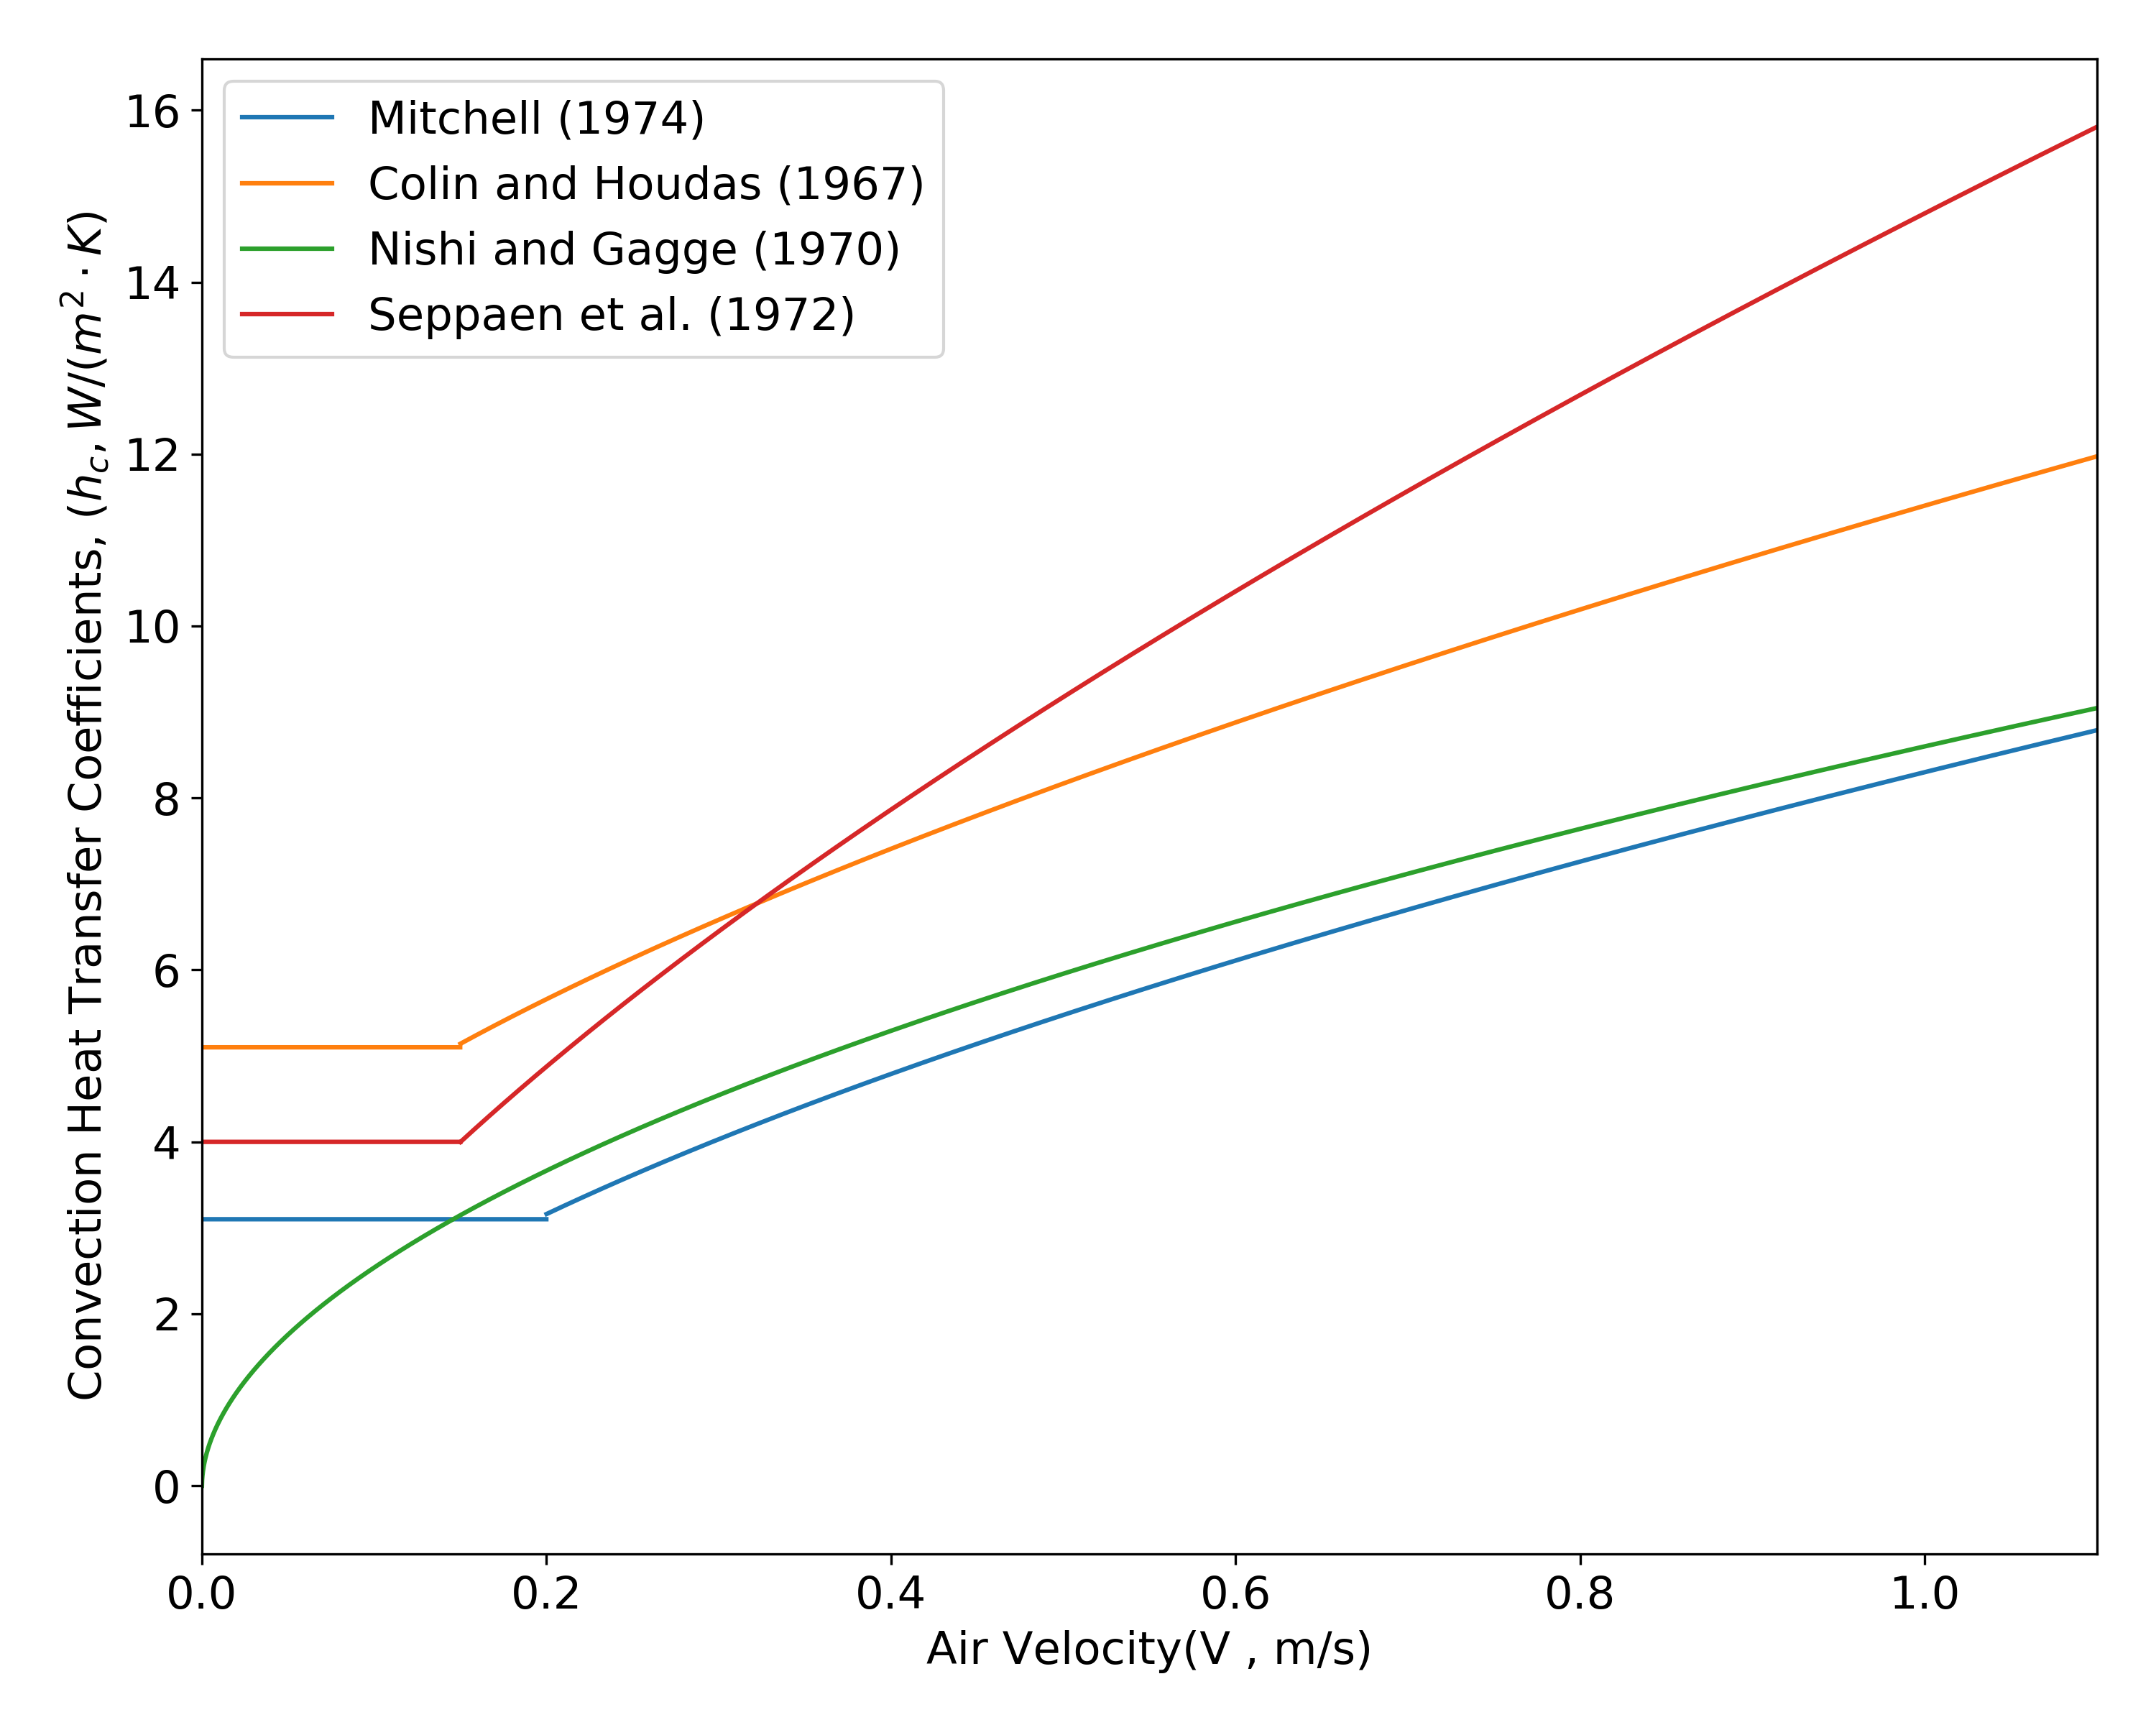
\includegraphics[width=0.5\textwidth]{figures/hcs4.png}
            \caption{$h_c$ with relation to air speed $V_a$ as defined in ASHRAE Handbook - Fundamentals 2009.}
            \label{fig:hc4s}
    \end{figure}
        %Operative temperature as the indicator of thermal comfort. Background and current range of applicable usages.
    Observing the relationship between the air velocity and resulting $h_c$, there is a very interesting relationship between the air velocity and the resulting operative temperature when substituting the expressions for $h_c$ in Table~\ref{tab:hcs} to Equation~\ref{eq:top}.
    \afterpage{\noindent
    \begin{figure}
            \centering
            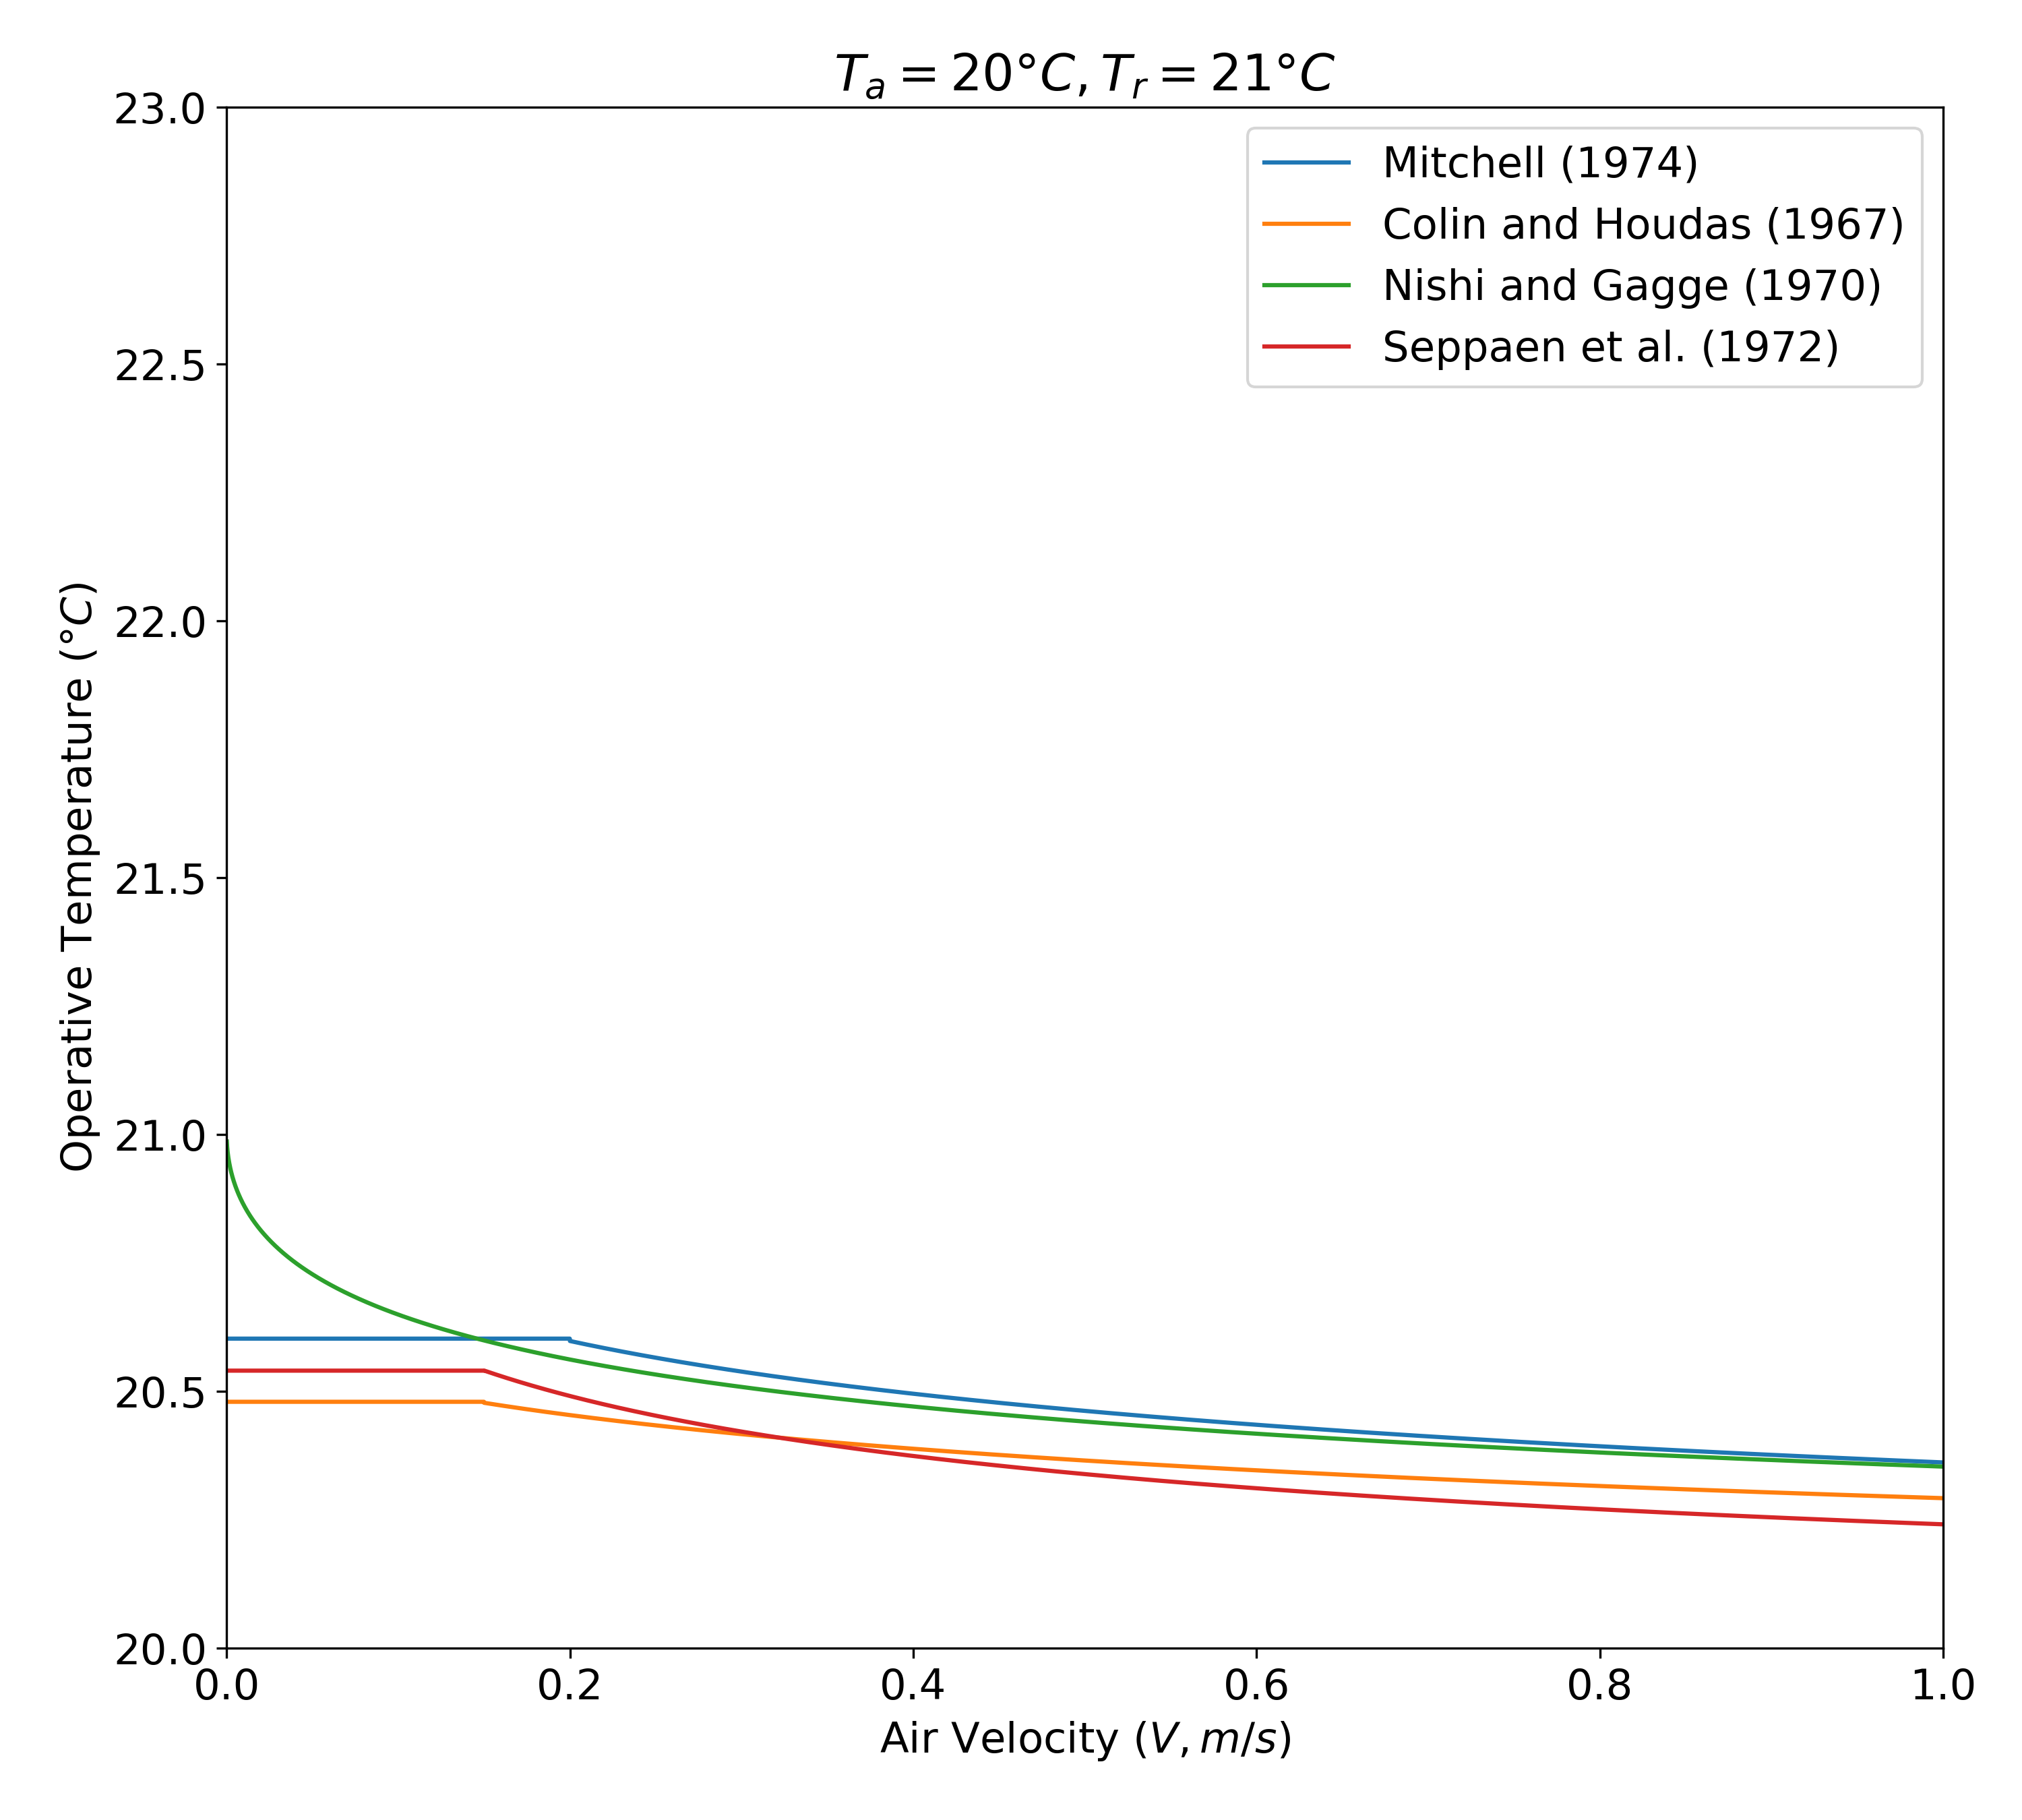
\includegraphics[width=0.49\textwidth]{figures/Ta20_Tr21.png}
            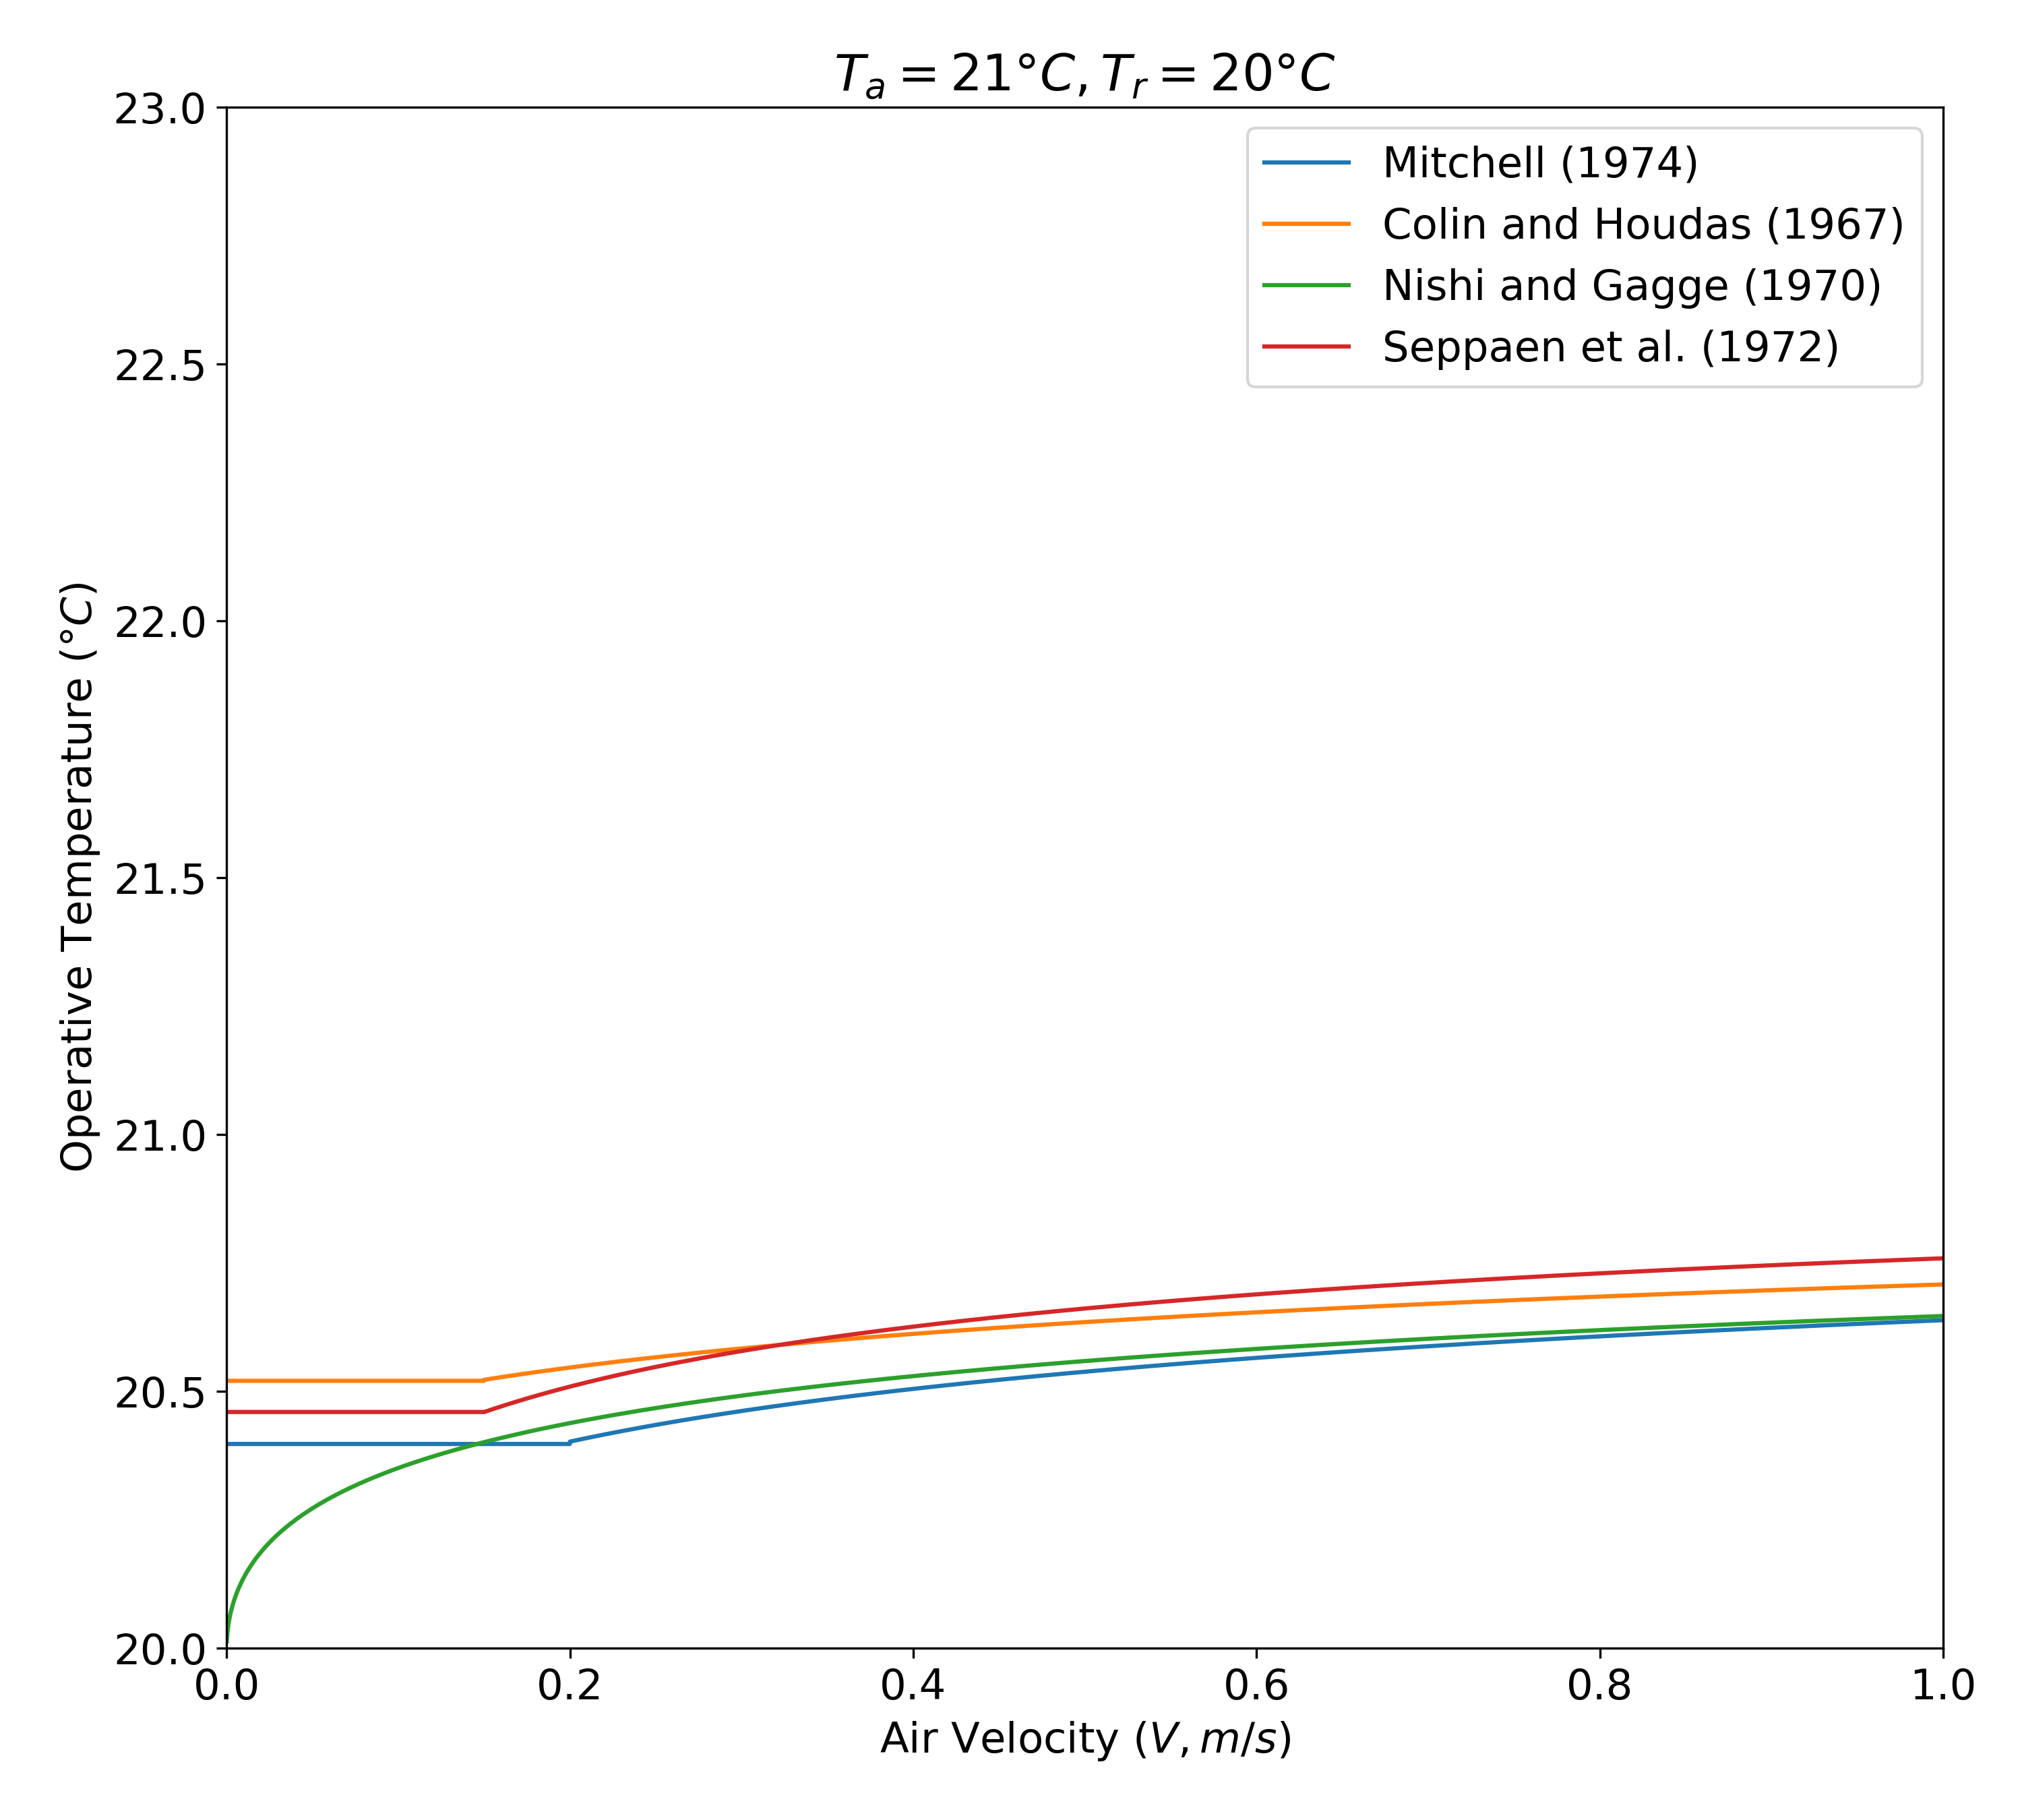
\includegraphics[width=0.49\textwidth]{figures/Ta21_Tr20.png}
            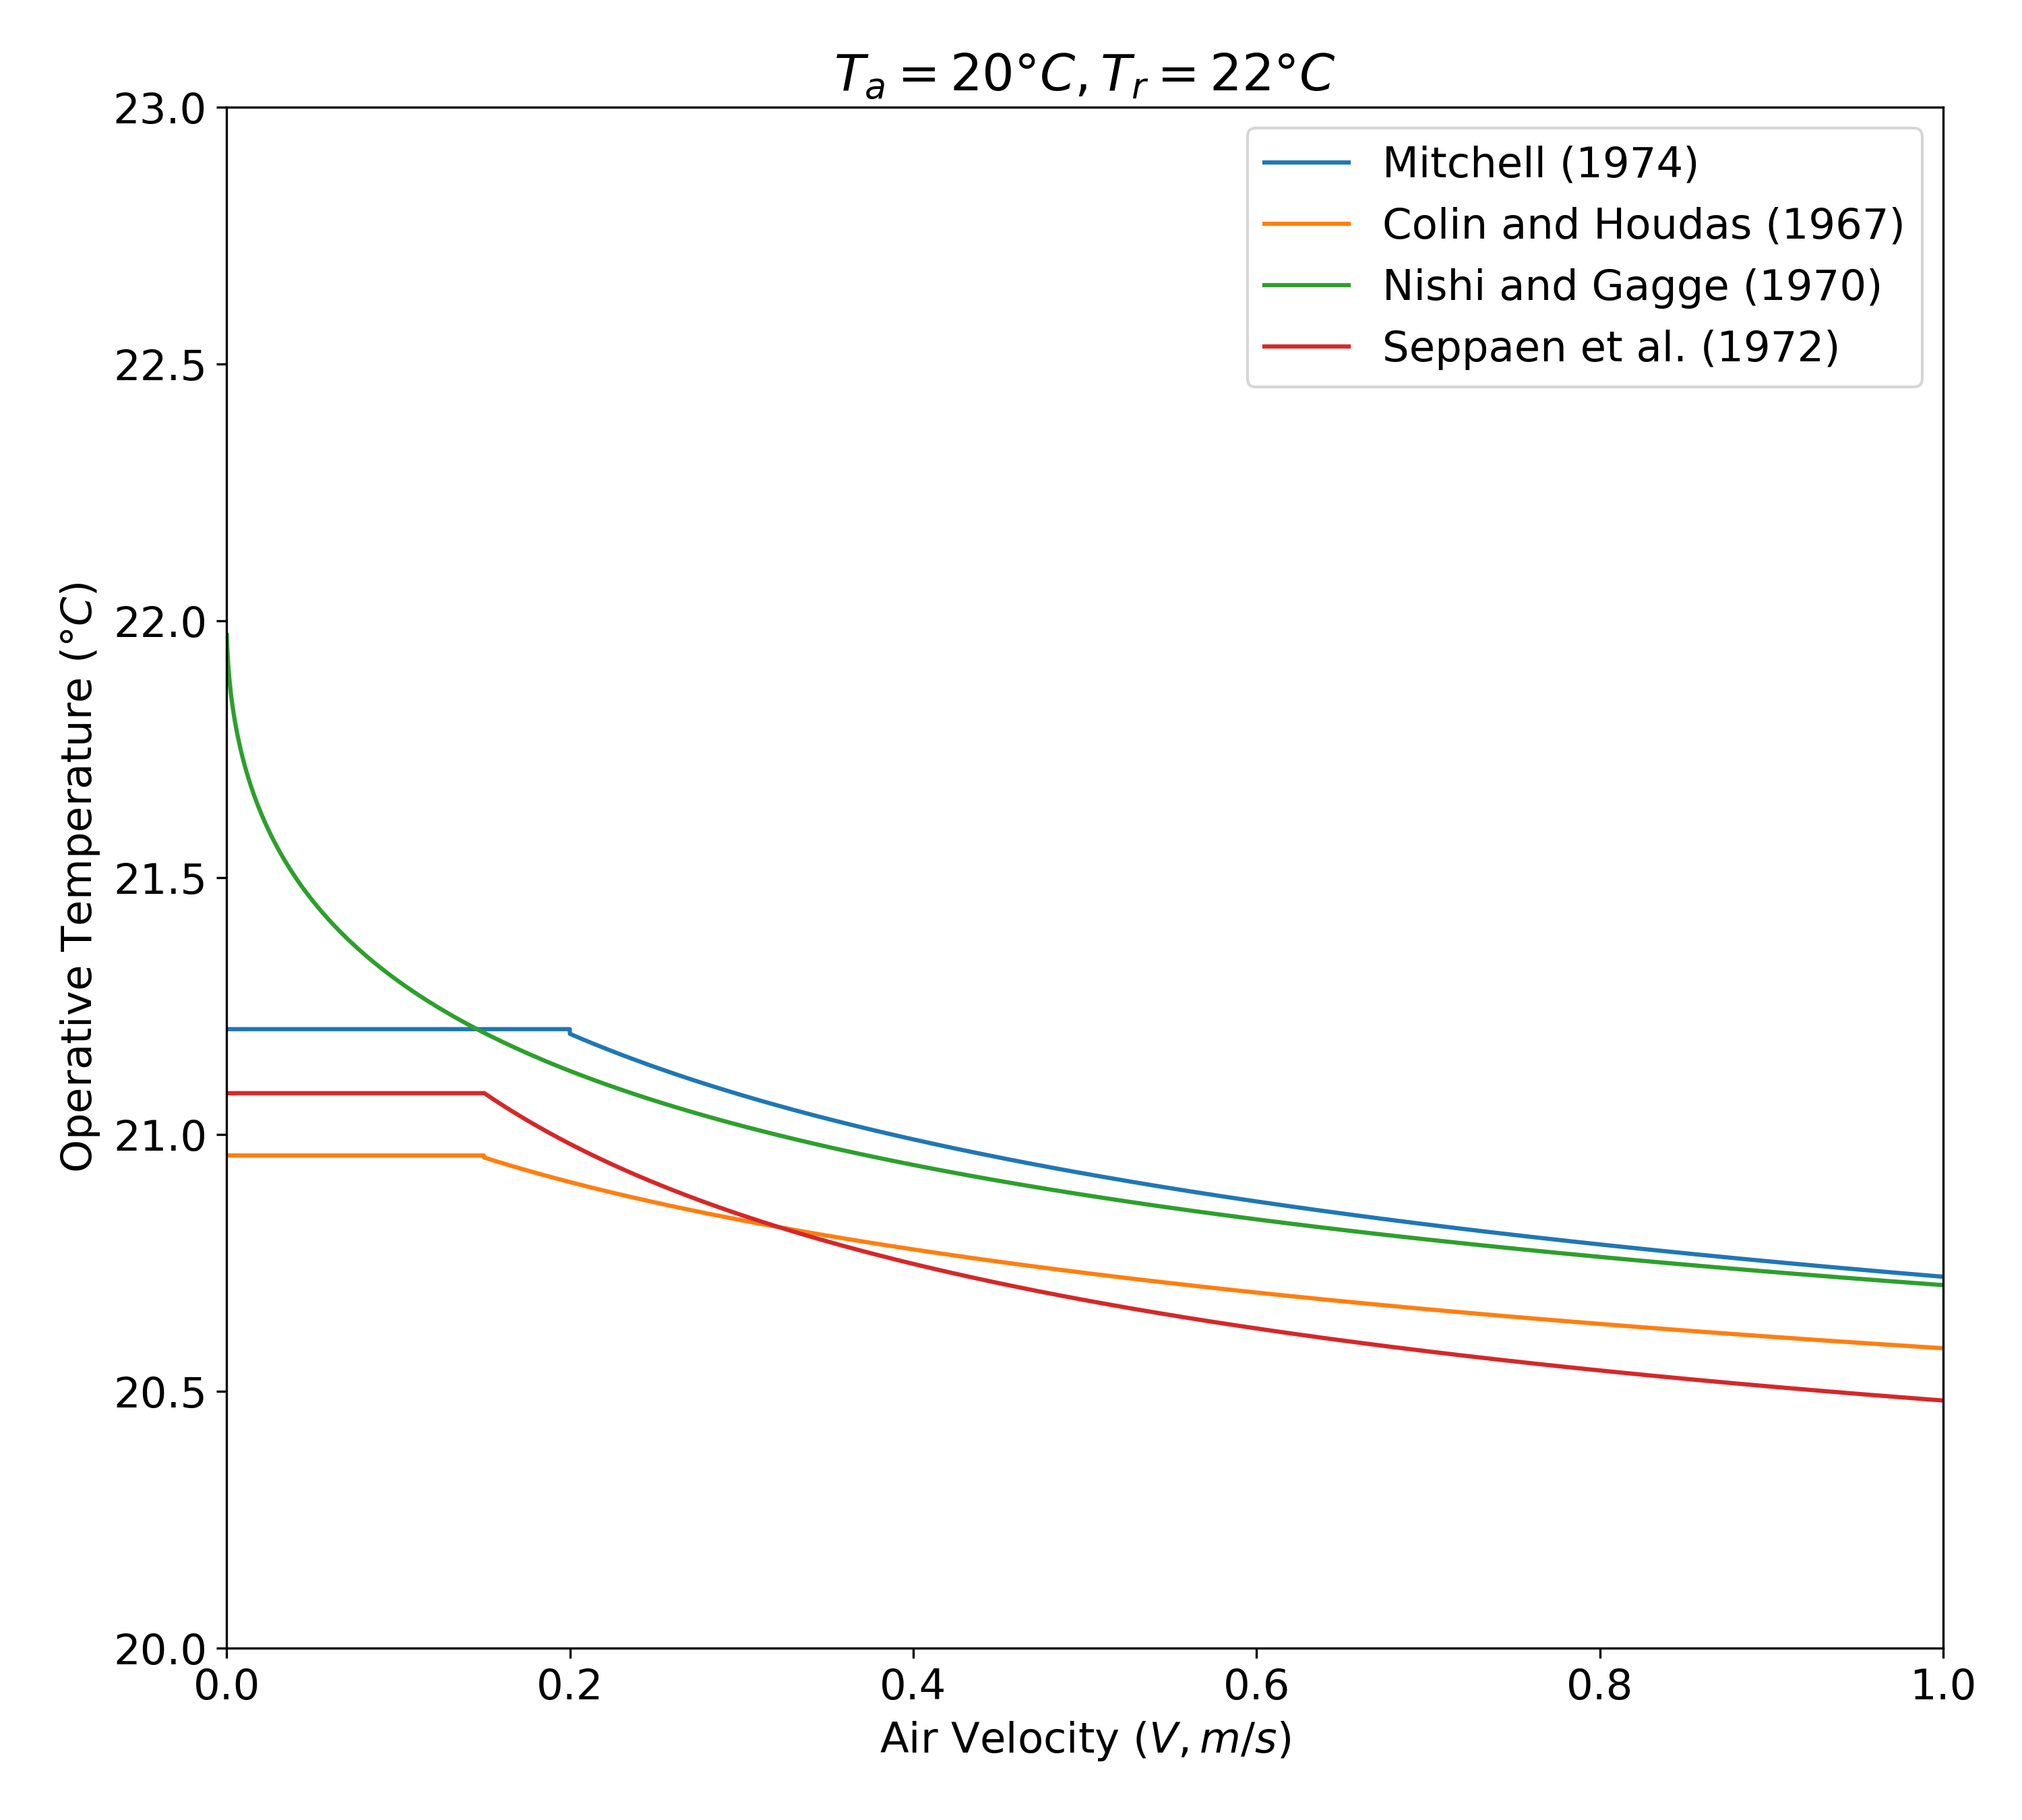
\includegraphics[width=0.49\textwidth]{figures/Ta20_Tr22.png}
            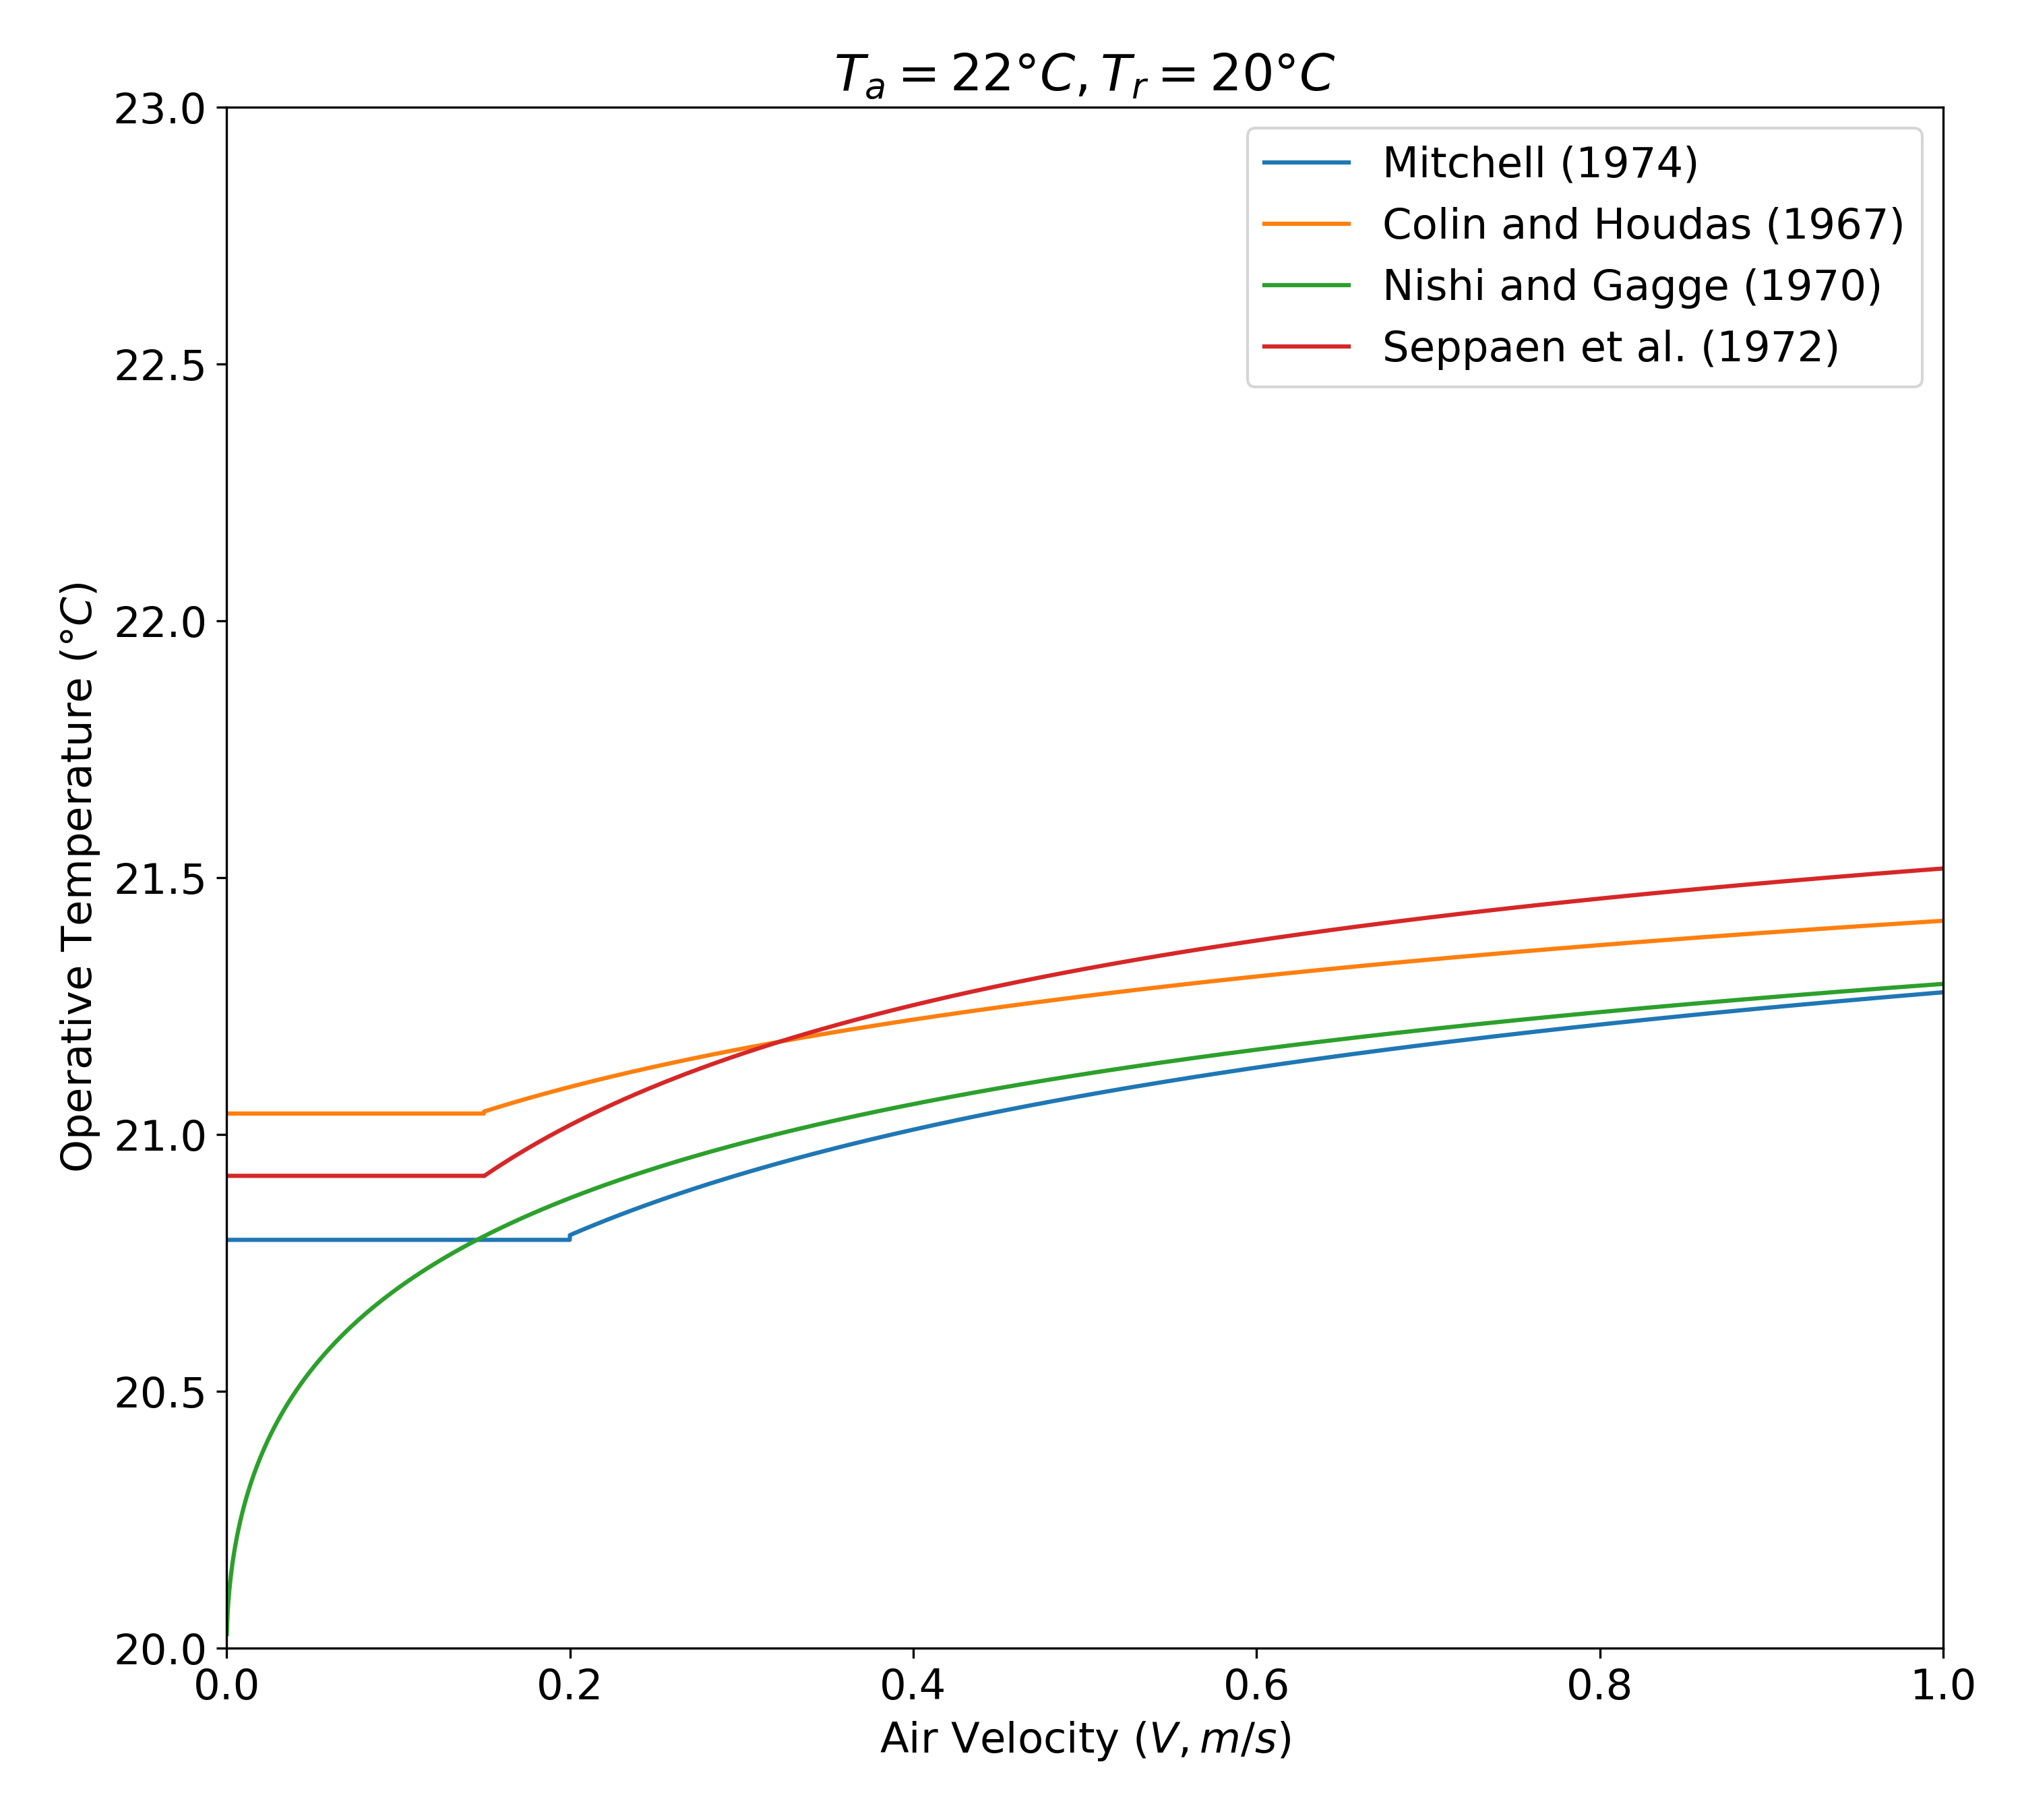
\includegraphics[width=0.49\textwidth]{figures/Ta22_Tr20.png}
            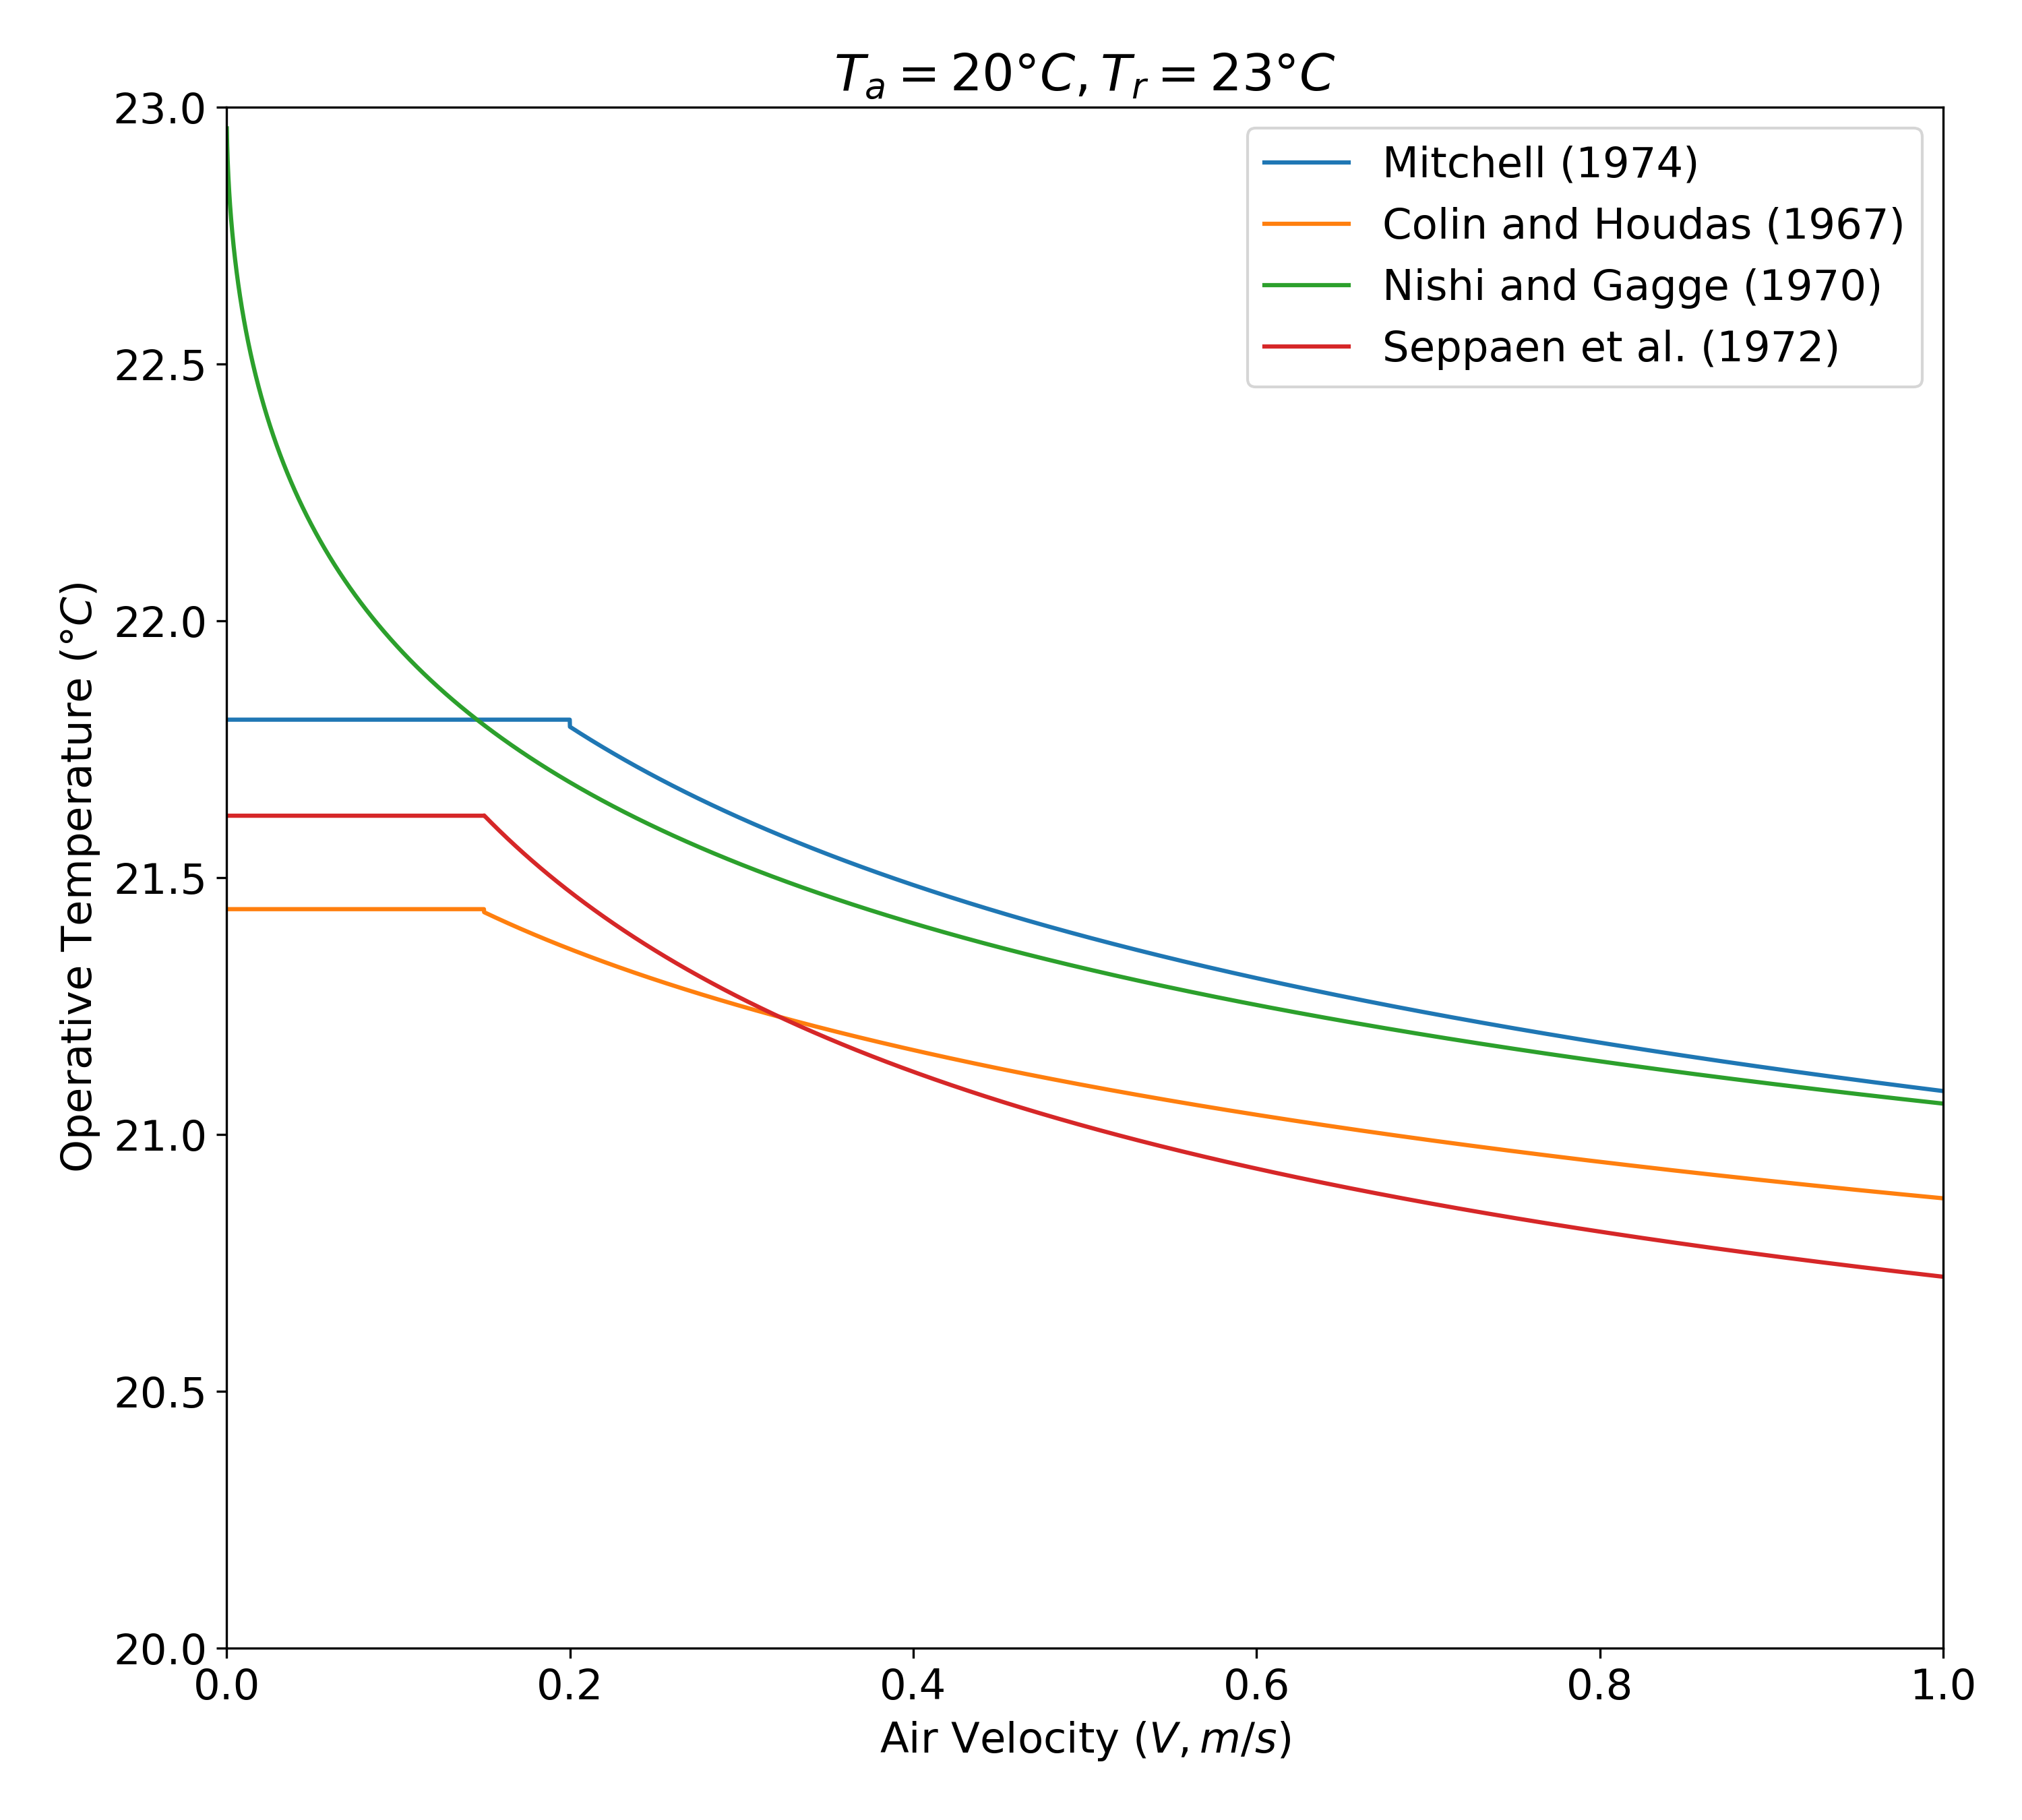
\includegraphics[width=0.49\textwidth]{figures/Ta20_Tr23.png}
            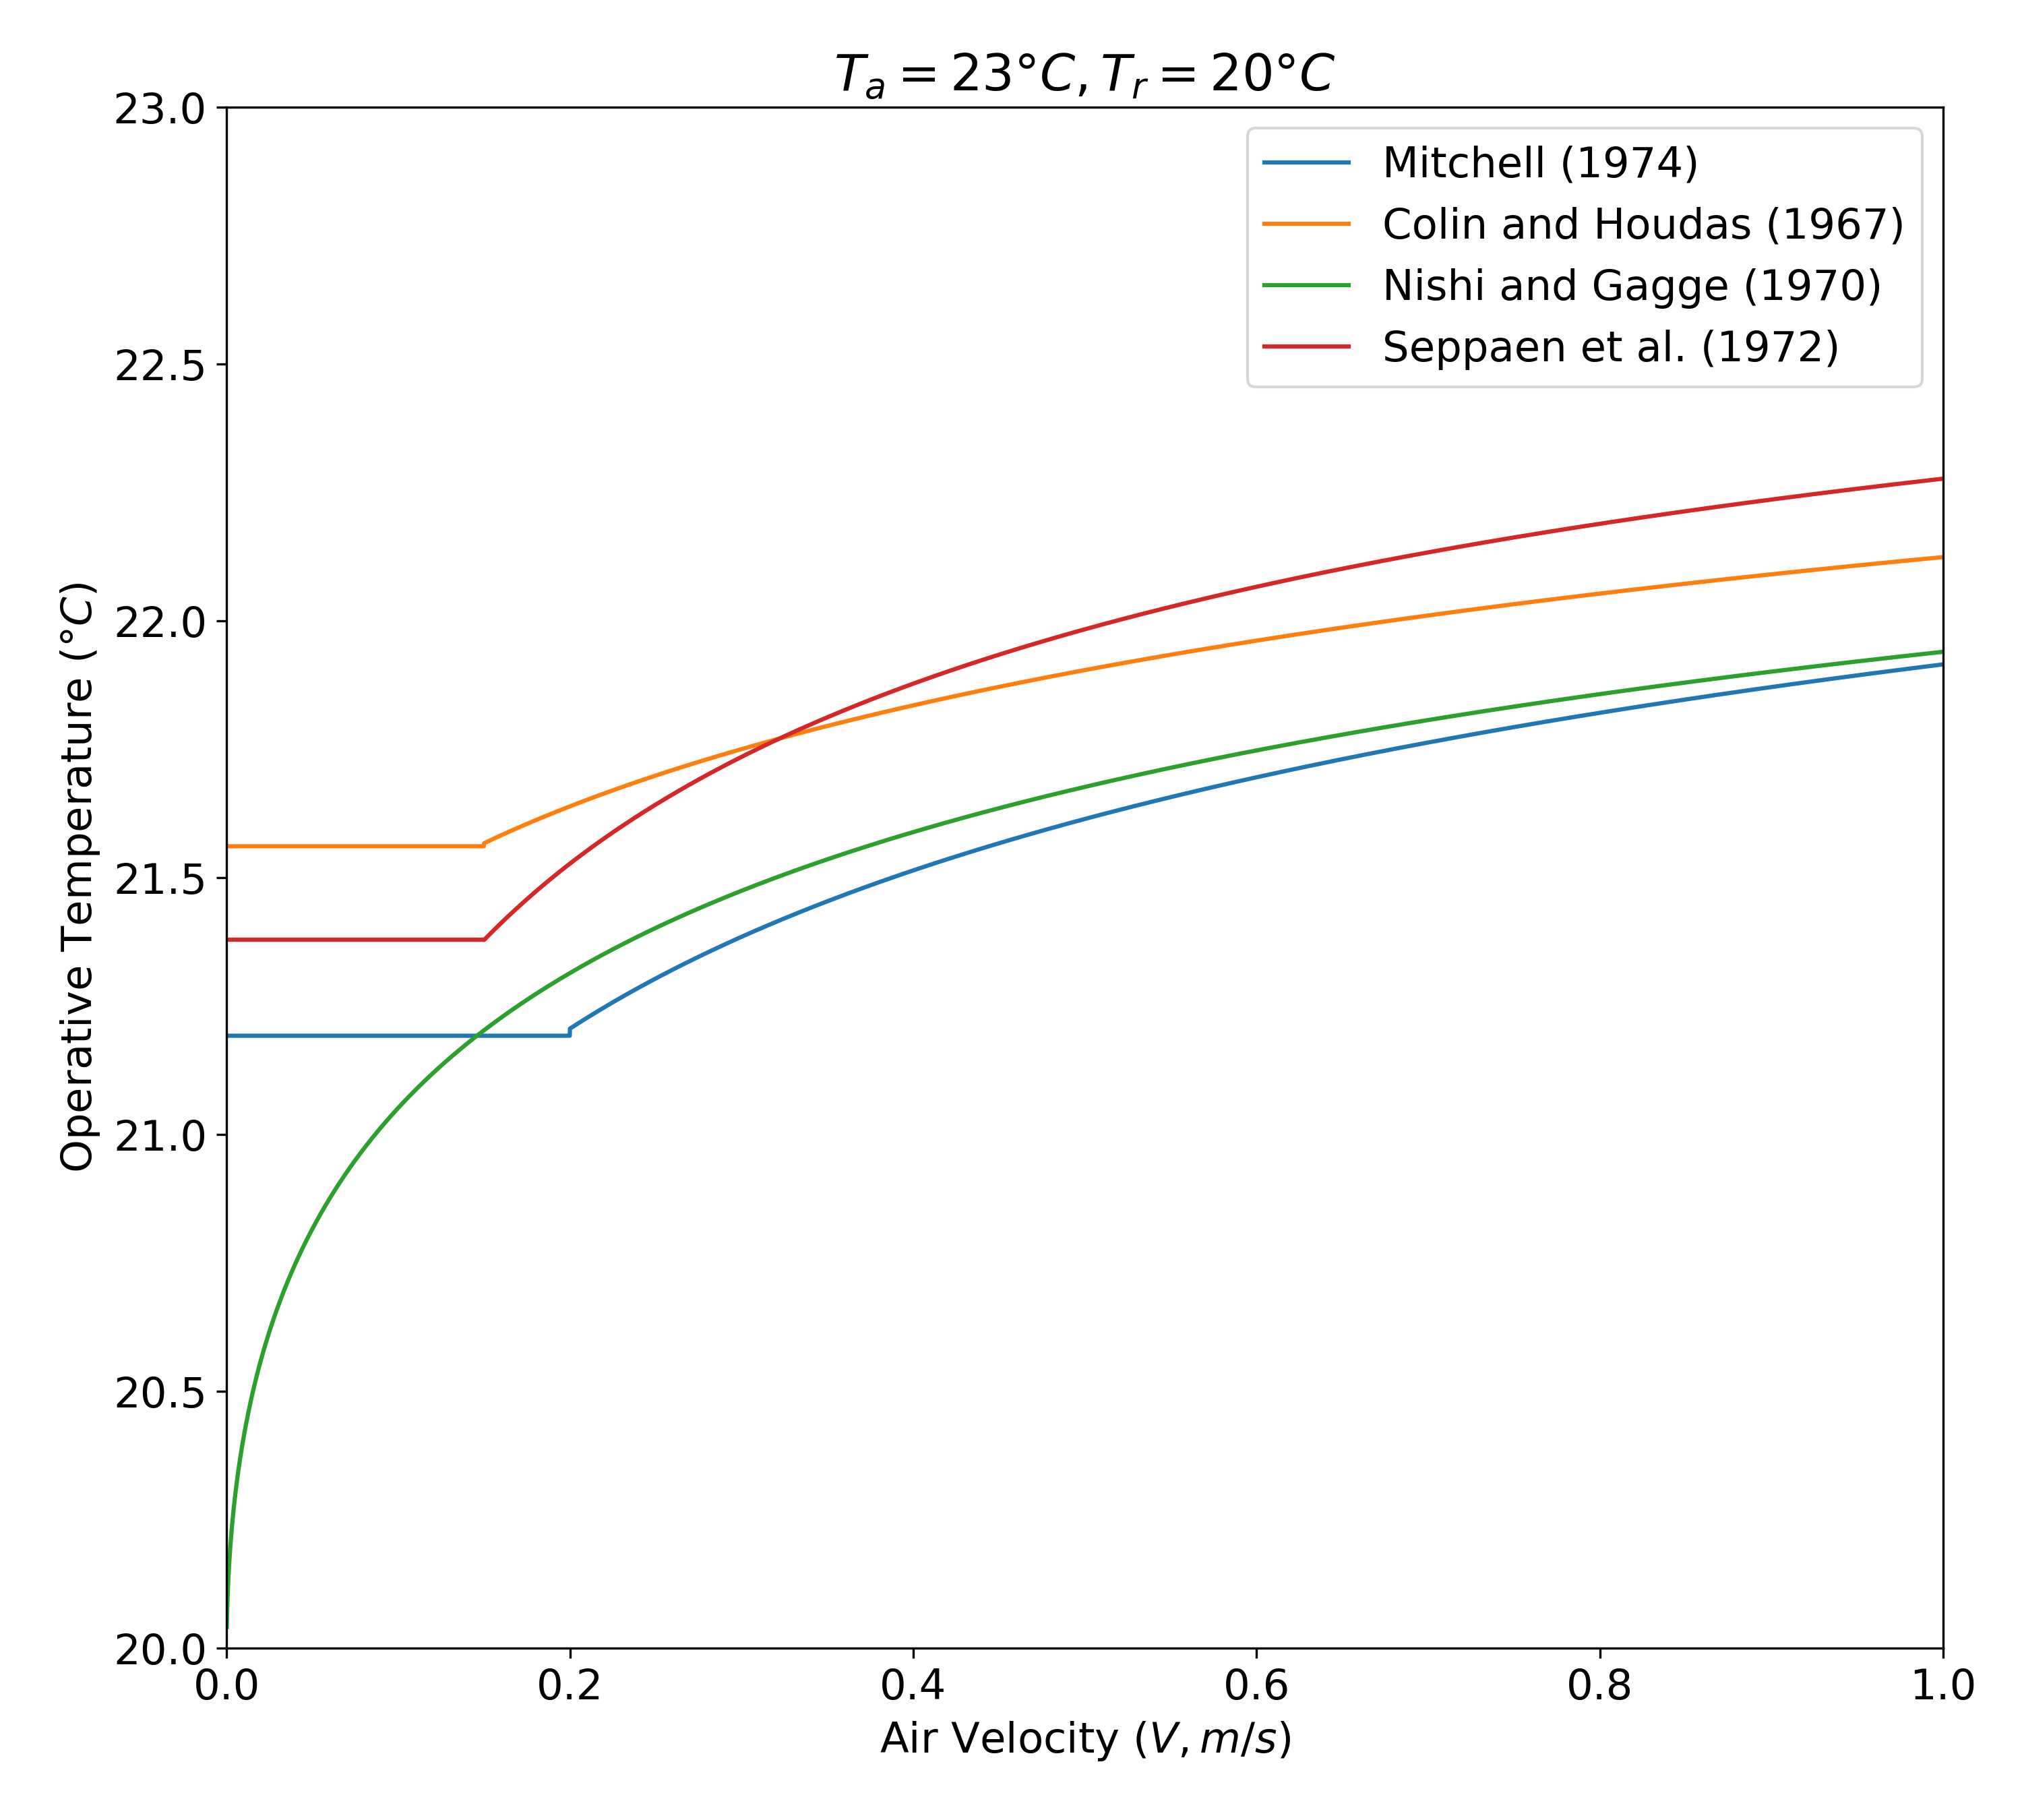
\includegraphics[width=0.49\textwidth]{figures/Ta23_Tr20.png}
            \caption{Relationship between air velocity ($V$) and operative temperature ($T_{op}$) when holding air temperature and mean radiant temperature constant.}
            \label{fig:Top_AR}
    \end{figure}
    }

    A very interesting phenomenon that we can observe, however, is the variation of operative temperature when holding air temperature and mean radiant temperature constant. As we're showing in Figure~\ref{fig:Top_AR}, increasing air velocity results in an increase of $T_{op}$ when $T_r$ < $T_a$, or a decrease of $T_{op}$ when $T_r$ > $T_a$.

    Alternatively, the definition of operative temperature as calculated per the formula given by ASHRAE 55-2017, where parameter $A$ is selected with respect to air velocity, or $V_a$. $A$ is evaluated at 0.5 when $V_a < 0.2m/s$, 0.6 when $V_a$ is between 0.2 and 0.6 $m/s$, and 0.7 when $V_a$ is between 0.6 and 1.0 $m/s$. As pointed out by SOMELIT, the overall clothing surface of a hypothetical average occupant is roughly 33.4 $\degree C$, thus any increase in $V_a$ when the ambient air temperature $T_a$ is below this number should be enhancing the convective heat transfer between the body and the surrounding environment, thus resulting in a decrease in perceived temperature. The operative temperature, in these cases, however, increases as the air velocity increases, which will result in the opposite direction of the prediction of thermal comfort. We believe this is a significant caveat of operative temperature to be used as a metric for thermal comfort assessment and would like to emphasize this in the current paper. More importantly, if we were to look back to the expression of operative temperature in Equation~\ref{eq:top}, it is evident that the definition itself is just a weighted average of air temperature and mean radiant temperature, which can easily become problematic when one of the heat transfer coefficient becomes much larger than the other - in this case $h_c > h_r$.

    Alternatively, the operative temperature can also be calculated from Equation~\ref{eq:opA55} to behave the same as indicated in Figure~\ref{fig:hc4s} where the operative temperature increases with increase of air velocity $V_a$ when $T_a > T_r$, which is the opposite of how an occupant exchanges heat with the surrounding environment as suggested by ASHRAE Standard 55-2017\cite{ansi/ashrae_standard_2017}. This will, again, not solve the effect of how higher $h_c$ influences
        \begin{equation}
            t_o = At_a + (1-A)\bar t_r\label{eq:opA55}
        \end{equation}

    Consequently, we believe there is a clear limitation of operative temperature to be used in indoor environment when radiant cooling is coupled with forced convection. Under scenarios created by such systems, the resulting operative temperature could be very misleading, i.e. increasing with the increase of air velocity despite the perceived temperature should have decreased for a hypothetical occupant. Examples that such a combination could exist are not uncommon:
    %DOAS + Chilled beam + forced convection? Open to examples!
\subsubsection{Predicted Mean Vote}
        Predicted Mean Vote (PMV) is a very popular concept in describing indoor thermal comfort. Developed in the 1970s, Fanger's  PMV model is based on both thermoregulation and heat balance theories as well as laboratory and climate chamber study results. The PMV model takes four physical variables (also referred to as environmental variables, i.e. $T_a$, $V_a$, MRT and relative humidity $\phi$) and personal variables (level of activity and clothing). Fanger's PMV model takes the six variables and produces a score that corresponds to the ASHRAE thermal sensation scale and represent the average thermal sensation felt by a large group of occupants \cite{ashrae_thermal_2003,fanger_thermal_1970}.

        There are some obvious benefits of using PMV. With the improvements in environmental control technologies, and the growth in personal wealth and office sizes (McIntyre, 1984), the need of better indoor environment requires a solution to predict the optimum temperature for a group of occupants, which can then be achieved by architects and engineers. Since its proposition in 1970, the PMV model has become the internationally accepted model for predicting and representing the mean thermal sensation vote by a large group of occupants for a set of given environmental variables. It has also since became the guideline for multiple international standards, where both ISO and ASHRAE indicated that a comfortable indoor environment can be insured when the PMV is kepted at 0 with a tolerace of $\pm0.5$.

        %Inidividual differences
        This does not mean there are not caveats in using PMV to describe the thermal sensation of offucpants. To begin with, there is an obvious difference in what Fanger's model can predict when compared to thermal comfort. As Fanger himself admitted, the usage of the heat balance models describes the balance between the thermoregulatory system and the environmental variables `even if comfort does not exist'. The neutral thermal sensation of an average person is not the same thing as thermal satisfaction, acceptability or preference. As Charles has pointed out in 1993, it is entirely possible for the occupants to vote on a neutral thermal sensation scale and to not feel comfortable.
        Neglecting the personal factors that reflects on their individual thermo-regulation and personal psychophysics is Natsume 1992, Havenith 2002

        %gender
        The PMV/PPD model also considers the inter-individual differences irrelevant from a series of experiments conducted in the 1960s. Fanger concluded from the results that the neutral temperature of a large group of occupants was independent of age, build, menstrual cycle, time of day, color and crowdedness of the room or gender, race as well as national geographic locations\cite{fanger_thermal_1970}. van Hoof pointed out that the original PMV model only accounts for the approximately 1,396 students who wear standardized clothes in a sedentary activity in Denmark, which does not reflect the larger and more diverse demographics of occupants in real buildings\cite{van_hoof_quantifying_2007}. Subsequent studies have since showed that there is a substantial gender differences where female occupants tend to feel significant cooler (Hill/Parsons 2002), and could be less satisfied with room temperatures while preferring higher room temperatures. Fanger made a similar observation earlier and concluded women are more sensitive to deviations than men\cite{fanger_assessment_1973}. To this observation, Parsons proceeded to conclude that during identical clothing and activity, the gender differences in thermal comfort responses for neutral and slightly warm conditions are smaller.

        %applicability
        The applicability of PMV has also became the subject of debate in some of the more recent publications. Despite some early validation of the PMV as a valid index when a meta-danalysis is performed, Humphreys and Nicol\cite{humphreys_validity_2002} found evidence of PMV bias often exceeding 0.25 scale units, and could reach as much as 1.0 - and the larger the deviation from neutral, the larger the bias. Their results suggested that PMV is only reliable between -0.5 and 0.5 unlike the range of validity stated by Fanger in his dissertation \cite{fanger_calculation_1967} and ISO (-2.0 and 2.0). More recently,  Cheong et al. found PMV only correctly predict thermal sensation correctly one out of three times\cite{cheong_local_2007}. This limitation of the PMV and PPD model is, however, not very well understood by practioners who are simply seeking a better metric and/or better adaptive model for conducting quick analysis of the thermal comfort requirements of an existing design. For practical purposes in existing projects, it is therefore highly desirable for practitioners to have a more accessible parameter to use for new and existing buildings, particularly when there are only limited information regarding the occupants and their schedules. %Setting pretext for adaptive thermal comfort

        %Thermal comfort zone
		%Regarding the thermal comfort zone - anlaytical tool?
		The latest standard published on determining the indoor occupants' thermal comfort is the ANSI/ASHRAE Standard 55-2017, which supersedes ANSI/ASHRAE Standard 55-2013, which is partially in agreement with ISO 7730, published as the ASRAE 55 Thermal Comfort Tool by the Center of Built Environment at Berkeley in 2017(Insert web citation).

		%What is comfort zone - it's verbal definition and graphical representation
		As briefly introduced previously, the comfort zone is defined as combinations of air temperature, mean radiant temperature $\bar t_r$  and humidity that are predicted to be an acceptable thermal environment at particular values of air speed, metabolic rate and clothing insulation $I_{cl}$(ASHRAE Standard 2017). It's also more commonly understood as two overlapping zones represented on psychrometric chart, where the air conditions are solved from a PMV of -0.5 to 0.5. This graphical approach assumes the rest of the environmental parameters (MRT, air velocity) and personal parameters (metabolic rate and clothing factors) as constants, and is the most widely accepted representation of the concept. There are actually two different ways of obtaining these boundary lines at PMV of -0.5 and 0.5. %Need to present it?

		%How we determine the comfort zone - three ways in ASHRAE.
		To determine the boundary of the comfort zone, both ISO 7730 and ASHRAE Standard 55 provide guidelines on how to do the actual calculation. There are currently three methods outlined in ASHRAE Standard 55, which applies to diffrent ranges of average air speed. With air speed lower than 0.2 m/s and a humidity ratio smaller than 0.012 kg$\cdot H_2O/kg$ dry air, the graphic comfort zone method should be used, where the operative temperature can be determined by linear interpolation the upper and lower operative temperature limit with a given clothing insulation. Alternatively, the comfort zone's boundaries can also be determined by using the Analytical Comfort Zone Method. This method can be applied to metabolic rate between 1.0 and 2.0, and clothing factor between 0 to 1.5 for all humidity ratios. This method incorporates the PMV calculation method used by ISO 7730.


        %Do we need to go so far for PPD? Probably unnecessary but it would hurt...
\subsubsection{The adaptive comfort model}
    The adaptive approach, first suggested by de Dear and Brager \cite{de_dear_developing_1998} was developed to account for the occupant adaptibility in environments that have wider bandwith than air-conditionined buildings such as naturally ventilated buildings. According to de Dear and Brager, the PMV model is not applicable for these environments because it only partly accounts for the adaptation process and were results from limited laboratory studies. They therefore proposed an adaptive thermal comfort model for free-runnign buildings, linking the neutral temperature indoors to the outdoor monthly average temperatures. According to van Hoof, Fanger responded to this model in 2004 by pointing out that adaptation should be `a process of machines adapting to human requirements and ergonomics, not the adaptation of humans to technology'\cite{van_hoof_forty_2008}, but this did not stop the expansion of the usage of the adaptive thermal comfort model in the subsequent studies. The adaptive thermal comfort is currently included in the ASHRAE Standard 55 as an optional method that can be applied to naturally ventilated office buildings when outdoor temperature is between 10 and 33 $\degree C$. %Consider adding in the equations for this - but only after adding in the equations for PMV also

    %How wide is this currently?
	As suggested by ASHARE Standard 55, the adaptive model applies to indoor environments with air speeds beyond 0.3 m/s, specifically where occupants have better control over their own built environment. Although not explicitly addressing the occupants in the room, this model appears to have worked well for scenarios including open offices, classrooms, and many other cases of natural or hybrid ventilation. 
    
    %What is the adaptive thermal comfort?
	However, it is important to point out that a majority of the laboratory studies that appeared to have demonstrated the usage of the adaptive thermal comfort models are more commonly found in studies conducted in classrooms among younger children - who exhibits not only higher metabolic rates, higher activity levels and smaller muscle/fat ratio. It is important to point out that these studies are more conclusive may not be a coicidence, i.e. that the younger occupants of an indoor environment. However, as these experiments are, in fact, conclusive, understanding their results are far more important than what was previously observed. %Younger,students, open plan offices

    %Some of its limitations?
    Despite some clear strength over the PMV/PPD models, the first limitation of the adaptive thermal comfort its exclusion of the six input parameters of PMV that regards the human heat balance as as crucial component to consider for the indoor environment.

    Comparing to the oeprative temperature and the predicted mean vote, the adaptive thermal comfort model is much less specific, since it is a non-deterministic metric. The exploration of this model is a branch that stems out from
    %It comes out from Fanger's acceptance that there is a range of environmental conditions that people are 'in general comfortable', while Fanger's own model points to a deterministic range of comfort.

    The adaptive thermal comfort model also has an equivalent definition of the `comfort zone' for naturally ventilated spaces\cite{ashrae_ansi/ashrae_2013}. As outlined in the ASHRAE Standard 55, the upper and lower 80\% accetability limit of the operative operative temperature can be calculated from its linear relationship with the prevailing daily outdoor air temperature. 
    %Also needs to refer to the human body exergy model, how it should be a range of exergy consumption rates that applies to the entire setup - or the lack thereof. We need to emphasize how important this is, and how we might be able to develop anything out of it. Specifically addressing these could require a single paragraph of the exergy consumption rate (alternative models?)

    \subsection{Outdoor} 
    % !TEX root = all.tex
With respect to how the thermal comfort can be characterized within a thermal environment, the existing literature often uses indoor/outdoor to categorize them(Rupp, 2015). This is a valid classification method when considering the environments to be either built (indoor) or natural (outdoor), which is also a natural result of the indoor and outdoor research communities being independent of each other: the indoor community focuses on ensuring the built environment satisfiable, following often either the ISO 7730 \cite{iso_iso_2005} or the ASHRAE Standard 55 \cite{ansi/ashrae_standard_2017} while the outdoor community deals with a wider range of environmental parameters and are often more concentrated on heat stresses ISO 7243 (7243, 2017). When it comes to the actual method of evaluation, we believe we can also categorize these thermal comfort metrics into whether they're directly measurable or not. Understanding whether resulting indices are directly linked to 

\subsubsection{Non-measurable metrics}
    A significant portion of the metrics used in the outdoor environment when assessing thermal comfort are not directly measurable
    %NOTE: THIS IS BEYOND OCCUPANT EVEN, as there's NO WAY to validate the simulated results other than their comparative differences, emphasize on how many different variables are involved during this process. 
    Among these variables, the physiologically equivalent temperature (PET) and the universal thermal climate index (UTCI) are becoming increasingly popular.
    \paragraph{PET} is first proposed by Hoppe who pointed out the necessity of a universal index describing the well-being of the occupant for both the indoor and outdoor environment. 
    
    benefits and caveats of PET
    

    The physiological equivalent temperature (PET) was proposed by Hoppe\cite{h._hoppe_new_1992}   
    \paragraph{UTCI}, or universal thermal climate index is a concept specifically developed by urban climatologists to address the challenges posed by the ongoing/upcoming challenges observed in the urban environment.
    %How it was first proposed
    
    Its application among the existing studies primarily sits within the urban climate studies and simulations.
    
    It's important to point out that all these metrics are non-measurable and unverifiable on their own. Unlike vote-like systems such as PMV that the results can directly be compared with the actual mean vote among the occupants, these variables cannot be compared with directly measured values without making assumptions about what is the best proxy of comfort. 
    Attempts to verify the simulated results often ends up  
    A common trait between these variables is that none of them can be actually measured or calibrated. 
\subsubsection{Measurable metrics}
        %W/m2
        W/m2
        $W/m^2$ is the surface-area-averaged incoming radiation at any given time. It can be directly measured by radiant flux sensors - often a thermopile (Jones, 1985). Thermopiles are capable of generating various votltages, thus by measuring the voltage differences generated between overall incoming radiant flux and the surrounding environment, and can therefore be used to measure the radiant flux within measured field of view. 
        
        WBGT -> wet bulb globe temperature
        MRT -> Application of globe thermometers


        %WBGT - any other metrics?

        %Globe Temperature

        %

\section{Common Simplifications and Assumptions found in the equivalence of thermal comfort}
    \subsection{Occupant-related Simplifications}
    The first and foremost simplification that we observe in the existing models of thermal comfort is how a group of occupants became a single occupant, or a synthetical one for that matter.

Fanger's research back in the 1970s were among the first to suggest that occupants can be represented by a single hypothetical occupant\cite{fanger_thermal_1970}. Based on his own deterministic thermoregulation-based model that calculates the absolute state of thermal comfort devleoped in 1967\cite{fanger_calculation_1967}, his dissertation asserts a calculated PMV within the range of -0.5 and +0.5 is sufficient to be representative of the entire population of any occupant group. Using experimental results collected from 1,394 college students, Fanger concluded that demographic variations among the occupants are not significant enough to affect the thermal comfort conditions. Although there are many further research suggesting otherwise\cite{kingma_energy_2015,wang_individual_2018}, the simplification of the occupants into a single occupant gradually became mainstream\cite{ansi/ashrae_standard_2017}.


\subsubsection{Outputs from the occupants}
        Physiological responses - why aren't they mesured?
        State of art
        Challenges in directly measuring physiological feedback of the human body

        Challenges for Using actual comfort votes as control feedback signal

\subsubsection{Inputs for individual occupants that haven't been modelled and or guaged}
	The first and perhaps the largest simplification among occupants is the metabolic rate. Following Fanger's proposition in 1967 \cite{fanger_calculation_1967}, the metabolic rate of the occupants has been assumed to be 58.2$W/m^2$, or 1 MET in most of the follow-up literatures and regulations, such as the ASHRAE Standard 55\cite{ashrae_ansi/ashrae_2013} and ISO 7730\cite{iso_iso_2005}. 
        Metabolic rate, clothing factor, age, build and sex are all ignored in conventional comfort modelling, where a middle-aged, medium-built hypothetical man is considered.

    \subsection{Environmental Parameters Simplifications}
    % !TEX root = all.tex    
    Defined as the temperature of a homogeneous sphere that exchanges the same amount of heat as the actual surrounding with the human body, mean radiant temperature is arguably the most problematic environmental parameter within both the indoor and outdoor environment \cite{kantor_most_2011}. Its definition is very easy to follow but difficult to compute, particularly due to the challenges of quantifying the view factors betwen the human body and the surrounding environments. In the meantime, mean radiant temperatures are required to calculate thermal comfort and heat stress indices such as the UTCI(Jendritzky, 2012), PT (Staiger, 2012), PET (Hoppe,1999) as well as PMV \cite{fanger_calculation_1967}. 

    Recent expansions of its definition to include the influence of the sun also add up to the challenge, as the mean radiant temperature now has two subsets with respect to the wavelength of the incoming radiation: longwave and shortwave\cite{ansi/ashrae_standard_2017}. Partially due to these inherent complexity of the mean radiant temperature, it is one of the most abstracted environmental parameter of all the environmental parameters. These simplifications are shared among existing standards (such as ISO 7726 \cite{standardization_iso7726_2001} and ASHRAE Standard 55 \cite{ansi/ashrae_standard_2017}) with both literal definitions and measurement techniques that are underlined with various simplifications. 
    \subsubsection{One MRT in one room}
        %Standards - 7726 and 55
    The first simplification for the mean radiant temperature that it is a room-specific variable. This simplification is very common among the existing literature and standards such as the ISO 7726\cite{standardization_iso7726_2001} and ASHRAE Standard 55. Within the ISO Standard, the thermal comfort ergonomics and its measurement was meant to be the focus. Despite acknowledging the  Standard 55 - 2017 from ASHRAE provided similar guidelines where the literal definitions of mean radiant temperature and the relationship between the long wave and shortwave radiations. 

    %Device-specific? Another layer of how MRT is understood.
    Problems in under MRT as a concept: difficulty to interpret Iterations attempting to simplify MRT: ISO, surface averaged, etc. Causes problems in measuring MRTs.

    %Fundamental difficulties of calclating the view factors? Direction of the human body? clothing surfaces, emissivity, etc.?
    Measurement protocols of MRT and IEQ (check PoE protocols).
    %Simulation methods when obtaining MRT(CBE MRT tool)
    Existing tools that evaluates the spatial variation of MRTs are also very rare. On the simulation side, the most common building simulation engines such as EnergyPlus \cite{energyplus_engineering_2013} do account for the temperature variations and calculate the respective view factors, but still remains to assess the mean radiant temperature as a single node inside a specific thermal zone despite accounting for the surrounding surface temperatures and their respective view factors. More recently, the Center for the Built Environment published a Spatial Thermal Comfort Tool \cite{arens_modeling_2015} that focuses on the spatial resolution of mean radiant temperature, which calculates both the spatial MRT and the corresponding PMV assuming constant inputs from the other five parameters ($T_a, v_a, RH, clo, M$).  
        
    The relationship between MRTs and the resulting PMVs have also been a subject of interests for many studies. 
\subsubsection{Air temperature and MRT}
        Aside from assuming that mean radiant temperatures can be treated as a homogeneous parameter for an indoor environment, another very common simplification is to consider mean radiant temperature the equivalent of air temperature\cite{kantor_most_2011}(Langer, 2013; matzarakis 2008). 
                Cases where this assumption might be true.
            Scenarios where Air IS NOT MRT needs to be better recognized:
            Radiant systems
            Shortwave radiation through huge fenestration systems
            Larger view-factors of adjacent cold/hot surface areas: ocean/river
\subsubsection{Simplified RH}
        Maybe briefly mention how we are suggesting we have already kept HR in check?
        Complexity in creating two-objective systems? Price?
% \subsection{Other sensed data}
%     A good(?) question is whether we want to keep the structure of the paper - or add more stuffs. There's the performance gap hat should go in somewhere, and problem of the two-stage simplification is that it's not super clear yet. How do you simplify a group into a person, that part is not clear enough. Or is it? In 3-1 and 3-2?

\subsection{Review of Recent Literature}
    To better understand how are these simplifications and assumptions affecting the status-quo research, we have also conducted a data-driven literature review, where we focus on finding the actual metrics measured in thermal comfort studies conducted since 2000 to 2020, as was identified by Park \& Nagy \cite{park_comprehensive_2018} to be relevant period of thermal comfort research. The challenge of manually reviewing the thermal comfort research that has been published over the last 20 years, we leveraged the free academic search engine demensions.ai to collect the bibliographical data including keywords, abstracts and citations and export them to be analyzed with TextBlob with Python after initial processing in VOSViewer. We selected dimensions.ai over other portals since it has a few key strengths over the more common databases like Google Scholar and Web of Science, as it contains not only more expanded journal publication records, but also grants, patents and policy documents. Using its dedicated API, more explicit requests for publication records are also possible. 

    %Method, WoS, Journal, data collection
    To collect the publication records for the purpose of this study, we used the search term \textit{"thermal comfort"} and \textit{"buildings"} to identify the whole pool of relevant research published between 2000 and 2020. The classification terms for the full literature dataset are respectively the six components contributing to thermal comfort are then used respectively \textit{"air temperature"}, \textit{"mean radiant temperature"}, \textit{"air velocity"}, \textit{"relative humidity"}, \textit{"clothing factor"} or \textit{"metabolic rate"} - as identified by Fanger in 1967\cite{fanger_calculation_1967}. 

    As a result, we identified 44,532 journal publications from the Dimensions engine of papers published between 2000 and 2010. We downloaded the metadata of the publication, including the title, abstract, author, citation, publicatin year for further analysis. This was collected between 586 journals, among which the most cited remains to be \textit{Building and Environment} and \textit{Energy and Buildings}, which was consistent with Park and Nagy's finding\cite{park_comprehensive_2018}. 
%To be depreciated into either a few paragraphs or completely buried in text, particularly the sensors. 
% \section{Tools used in determining state of thermal comfort}
%         \subsection{Apparatus}
%         \input{4_1_tools_apparatus.tex}
%         \subsection{Analytical tools - the comfort zones}        
%         \input{4_2_tools_anaCZ.tex}
\section{Latest Efforts in addressing the absence of occupant in OCC}
%Regarding the 2nd level of abstraction: how this is further emphasised improved into the buildings later. 
Despite all the implicit assumptions and simplifications within the existing models, there have already been attempts to address the challenge of thermal comfort among multiple occupants. To address the challenge of satisfying occupants of different demographic/physiological conditions, these efforts share an important trait of including actual occupants responses, but can be further catgorized into two groups: those that include only the subjective feedback from the occupants, and those that also include the objective measurements of the occupants\cite{bortolini_analysis_2019}. Although both categories aims at collecting feedback from the occupants, they essentially are addressing different aspect of the problem through voluntary and involuntary feedback from the occupants. Ideally, the feedbacks should always be involuntary since the interruption to the workflow or activities of the occupants can be kept to the minimum level. 
    \subsection{Subjective feedback}
    We categorize studies that uses the subjective votes without direct physiological measurements as subjective. Occupants are no longer providing involuntary feedback but rather intentional, voluntary responses as signals collected by the control system or algorithm. 

%Preferences, sensations, etc. 

%But can we consider preferences also as objective? Due to the individual differences, or variations of the metabolic rates?




%Regarding the thermal comfort zone - anlaytical tool?
The latest standard published on determining the indoor occupants' thermal comfort is the ANSI/ASHRAE Standard 55-2017, which supersedes ANSI/ASHRAE Standard 55-2013, which is partially in agreement with ISO 7730, published as the ASRAE 55 Thermal Comfort Tool by the Center of Built Environment at Berkeley in 2017(Insert web citation). 

%What is comfort zone - it's verbal definition and graphical representation
As briefly introduced previously, the comfort zone is defined as combinations of air temperature, mean radiant temperature $\bar t_r$  and humidity that are predicted to be an acceptable thermal environment at particular values of air speed, metabolic rate and clothing insulation $I_{cl}$(ASHRAE Standard 2017). It's also more commonly understood as two overlapping zones represented on psychrometric chart, where the air conditions are solved from a PMV of -0.5 to 0.5. This graphical approach assumes the rest of the environmental parameters (MRT, air velocity) and personal parameters (metabolic rate and clothing factors) as constants, and is the most widely accepted representation of the concept. There are actually two different ways of obtaining these boundary lines at PMV of -0.5 and 0.5. %Need to present it?

%How we determine the comfort zone - three ways in ASHRAE.
To determine the boundary of the comfort zone, both ISO 7730 and ASHRAE Standard 55 provide guidelines on how to do the actual calculation. There are currently three methods outlined in ASHRAE Standard 55, which applies to diffrent ranges of average air speed. With air speed lower than 0.2 m/s and a humidity ratio smaller than 0.012 kg$\cdot H_2O/kg$ dry air, the graphic comfort zone method should be used, where the operative temperature can be determined by linear interpolation the upper and lower operative temperature limit with a given clothing insulation. Alternatively, the comfort zone's boundaries can also be determined by using the Analytical Comfort Zone Method. This method can be applied to metabolic rate between 1.0 and 2.0, and clothing factor between 0 to 1.5 for all humidity ratios. This method incorporates the PMV calculation method used by ISO 7730.
    \subsection{Objective measurement}
    Regarding the latest research focusing on addressing the two-step simplification of occupants into environmental parameters, we can categorize them based on their means of planned intervention and its relationship to the occupants into objective and subjective. For the objective interventions, occupants' physiological responses are directly measured through different sensing techniques, and calibrated by the actual votes of the occupants. 

\subsubection{Skin temperature and IoT}
Measuring the physiological response of the human body has been historically challenging. 

Among other measurable responses, the skin temperature of the human body is more common in existing research. To accurately measure the physiological responses of the human body, traditional sensing techniques are often intrusive: sensors that needs to be strapped onto the body \cite{mccarthy_validation_2016}, or needing to be ingested (pill-type, update citation) effectively make it impossible to measure real-time responses for multiple multiples in a real office environment. 

Development in sensing technology has helped researchers to come up with solutions to the comfort conundrum. 

Studies on how sensitive different locations of the human skin are sensitive to changes of the thermal environment have pointed skin temperature to be \cite{choi_cobi:_2010}

? Occupancy, infrared-based occupancy sensing? Can we suggest that is also measuring 
\subsubsection{Thermal Imagery and other direct measurement techniques}

% \subsubsection{Globe Thermometer}
%             It’s first introduction (indoor)
%             Limitations recognized - and simplification introduced
%             One MRT per room.
%             Proliferation/increase of its usage (citations? How do we quantify its virus-like applications within both the indoor and outdoor environment)
%             Linkage to Top - (Do we want to discuss the relationship between Top and the convection here?)
%             prior.
            
% \subsubsection{Net Radiometer}
%             Outdoor introduction
%             Expenses, immobilized
%             Marty as being mobilized - CITATIONS
%             Less commonly used since introduction of globe thermometers
            
% \subsubsection{Operative temperature sensors}
%                 Globe thermometers >10
% \subsubsection{Air Temperature Sensors}
%                 Less documented but more often used in real systems.
%                 Air = MRT as a simplification built beyond One MRT per room.
  
        %Check Kim's research on this? Where are the direct or indirect measurement coming in? Debugging is/should always be about finding the bug, about knowing its existence is no accident. 
        \subsection{Occupant-centric building control}
        %Should be fairly easy as we're just including the June publication back here... but maybe not. 
        \subsection{Personalized thermal comfort model}
        
% \section{Results and Discussions}
\section{Conclusion}
We reviewed some of the most canonical parameters for thermal comfort in this paper, focusing particularly on their limitations and underlying simplifications. Our hypothesis of the occupants as larger groups went through a two-step simplification process was verified, upon which we also identified some of the most recent efforts to address the thermal comfort gap - which we believe is caused by the negligence of both the individual differences between occupants and the human physiological responses.

We discovered many problems in the existing simplification methods from a group of occupants to a single hypothetical occupant - it is not to say that the occupants cannot/should not be simplified, but the context of this simplification needs to be better undrstood among researchers and practitioners.

We also feel we need to better undrestand what and how many of thosesimplifications are used when their resuls are cited and used elsewhere. Many of the assumptions were passed on alongside their cited results. This also affects the data-drive approach when reviewing these papers, since the underlying assumptions will again go unexamined, and the asumptions get passed on without being re-examined.

Using direct methods to collect the outputs from occupants may be an alternative that could solve the comfort gap. Existing research in this direction uses either direct physiological measurements or actual feedback from the occupants, which can both be viewed as attempts to re-introduce the occupants back to the control loop of building systems. Other efforts includes the status-quo research on personal thermal comfort models that characterizes the individual thermal differences, which includes both the physiological feedback and the actual votes from the occupants. We believe personalized thermal comfort model is a promising alternative to the existing comfort/occupent-centric explorations, despite their limited scale at the time of this paper. 


To re-introduce the occupants to monitoring and control of indoor environment, it is necessary

We wanted to focus primarily on the two step abstraction of the thermal comfort of occupants in this paper and concentrated on how different simplifications and assumptions chronologically emerged during this simplification. This is further coupled with investigation on how recent awareness of the importance of thermal comfort. Whata re some of the basic traits of C++ as a language? How is this practical - or non-practical is a key problem that we're currently facing. 

\bibliography{top.bib}
\end{document}